% A LaTeX template for MSc Thesis submissions to 
% Politecnico di Milano (PoliMi) - School of Industrial and Information Engineering
%
% S. Bonetti, A. Gruttadauria, G. Mescolini, A. Zingaro
% e-mail: template-tesi-ingind@polimi.it
%
% Last Revision: October 2021
%
% Copyright 2021 Politecnico di Milano, Italy. NC-BY

\documentclass{Configuration_Files/PoliMi3i_thesis}

%------------------------------------------------------------------------------
%	REQUIRED PACKAGES AND  CONFIGURATIONS
%------------------------------------------------------------------------------

% CONFIGURATIONS
\usepackage{parskip} % For paragraph layout
\usepackage{setspace} % For using single or double spacing
\usepackage{emptypage} % To insert empty pages
\usepackage{multicol} % To write in multiple columns (executive summary)
\setlength\columnsep{15pt} % Column separation in executive summary
\setlength\parindent{0pt} % Indentation
\raggedbottom  

% PACKAGES FOR TITLES
\usepackage{titlesec}
% \titlespacing{\section}{left spacing}{before spacing}{after spacing}
\titlespacing{\section}{0pt}{3.3ex}{2ex}
\titlespacing{\subsection}{0pt}{3.3ex}{1.65ex}
\titlespacing{\subsubsection}{0pt}{3.3ex}{1ex}
\usepackage{color}

% PACKAGES FOR LANGUAGE AND FONT
\usepackage[english]{babel} % The document is in English  
\usepackage[utf8]{inputenc} % UTF8 encoding
\usepackage[T1]{fontenc} % Font encoding
\usepackage[11pt]{moresize} % Big fonts

% PACKAGES FOR IMAGES
\usepackage{graphicx}
\usepackage{transparent} % Enables transparent images
\usepackage{eso-pic} % For the background picture on the title page
\usepackage{subfig} % Numbered and caption subfigures using \subfloat.
\usepackage{tikz} % A package for high-quality hand-made figures.
\usetikzlibrary{positioning, shapes.geometric, arrows.meta, fit}
\graphicspath{{./Images/}} % Directory of the images
\usepackage{caption} % Coloured captions
\usepackage{xcolor} % Coloured captions
\usepackage{amsthm,thmtools,xcolor} % Coloured "Theorem"
\usepackage{float}

% STANDARD MATH PACKAGES
\usepackage{amsmath}
\usepackage{amsthm}
\usepackage{amssymb}
\usepackage{amsfonts}
\usepackage{bm}
\usepackage[overload]{empheq} % For braced-style systems of equations.
\usepackage{fix-cm} % To override original LaTeX restrictions on sizes

% PACKAGES FOR TABLES
\usepackage{tabularx}
\usepackage{longtable} % Tables that can span several pages
\usepackage{colortbl}

% PACKAGES FOR ALGORITHMS (PSEUDO-CODE)
\usepackage{algorithm}
\usepackage{algorithmic}

% PACKAGES FOR REFERENCES & BIBLIOGRAPHY
\usepackage[colorlinks=true,linkcolor=black,anchorcolor=black,citecolor=black,filecolor=black,menucolor=black,runcolor=black,urlcolor=black]{hyperref} % Adds clickable links at references
\usepackage{cleveref}
\usepackage[square, numbers, sort&compress]{natbib} % Square brackets, citing references with numbers, citations sorted by appearance in the text and compressed
\bibliographystyle{abbrvnat} % You may use a different style adapted to your field

% OTHER PACKAGES
\usepackage{pdfpages} % To include a pdf file
\usepackage{afterpage}
\usepackage{lipsum} % DUMMY PACKAGE
\usepackage{fancyhdr} % For the headers
\fancyhf{}

% Input of configuration file. Do not change config.tex file unless you really know what you are doing. 
% Define blue color typical of polimi
\definecolor{bluepoli}{cmyk}{0.4,0.1,0,0.4}

% Custom theorem environments
\declaretheoremstyle[
  headfont=\color{bluepoli}\normalfont\bfseries,
  bodyfont=\color{black}\normalfont\itshape,
]{colored}

% Set-up caption colors
\captionsetup[figure]{labelfont={color=bluepoli}} % Set colour of the captions
\captionsetup[table]{labelfont={color=bluepoli}} % Set colour of the captions
\captionsetup[algorithm]{labelfont={color=bluepoli}} % Set colour of the captions

\theoremstyle{colored}
\newtheorem{theorem}{Theorem}[chapter]
\newtheorem{proposition}{Proposition}[chapter]

% Enhances the features of the standard "table" and "tabular" environments.
\newcommand\T{\rule{0pt}{2.6ex}}
\newcommand\B{\rule[-1.2ex]{0pt}{0pt}}

% Pseudo-code algorithm descriptions.
\newcounter{algsubstate}
\renewcommand{\thealgsubstate}{\alph{algsubstate}}
\newenvironment{algsubstates}
  {\setcounter{algsubstate}{0}%
   \renewcommand{\STATE}{%
     \stepcounter{algsubstate}%
     \Statex {\small\thealgsubstate:}\space}}
  {}

% New font size
\newcommand\numfontsize{\@setfontsize\Huge{200}{60}}

% Title format: chapter
\titleformat{\chapter}[hang]{
\fontsize{50}{20}\selectfont\bfseries\filright}{\textcolor{bluepoli} \thechapter\hsp\hspace{2mm}\textcolor{bluepoli}{|   }\hsp}{0pt}{\huge\bfseries \textcolor{bluepoli}
}

% Title format: section
\titleformat{\section}
{\color{bluepoli}\normalfont\Large\bfseries}
{\color{bluepoli}\thesection.}{1em}{}

% Title format: subsection
\titleformat{\subsection}
{\color{bluepoli}\normalfont\large\bfseries}
{\color{bluepoli}\thesubsection.}{1em}{}

% Title format: subsubsection
\titleformat{\subsubsection}
{\color{bluepoli}\normalfont\large\bfseries}
{\color{bluepoli}\thesubsubsection.}{1em}{}

% Shortening for setting no horizontal-spacing
\newcommand{\hsp}{\hspace{0pt}}

\makeatletter
% Renewcommand: cleardoublepage including the background pic
\renewcommand*\cleardoublepage{%
  \clearpage\if@twoside\ifodd\c@page\else
  \null
  \AddToShipoutPicture*{\BackgroundPic}
  \thispagestyle{empty}%
  \newpage
  \if@twocolumn\hbox{}\newpage\fi\fi\fi}
\makeatother

%For correctly numbering algorithms
\numberwithin{algorithm}{chapter}

%----------------------------------------------------------------------------
%	NEW COMMANDS DEFINED
%----------------------------------------------------------------------------

% EXAMPLES OF NEW COMMANDS
\newcommand{\bea}{\begin{eqnarray}} % Shortcut for equation arrays
\newcommand{\eea}{\end{eqnarray}}
\newcommand{\e}[1]{\times 10^{#1}}  % Powers of 10 notation

%----------------------------------------------------------------------------
%	ADD YOUR PACKAGES (be careful of package interaction)
%----------------------------------------------------------------------------

%----------------------------------------------------------------------------
%	ADD YOUR DEFINITIONS AND COMMANDS (be careful of existing commands)
%----------------------------------------------------------------------------

%----------------------------------------------------------------------------
%	BEGIN OF YOUR DOCUMENT
%----------------------------------------------------------------------------

\begin{document}

\fancypagestyle{plain}{%
	\fancyhf{} % Clear all header and footer fields
	\fancyhead[RO,RE]{\thepage} %RO=right odd, RE=right even
	\renewcommand{\headrulewidth}{0pt}
	\renewcommand{\footrulewidth}{0pt}}

%----------------------------------------------------------------------------
%	TITLE PAGE
%----------------------------------------------------------------------------

\pagestyle{empty} % No page numbers
\frontmatter % Use roman page numbering style (i, ii, iii, iv...) for the preamble pages

\puttitle{
	title=Explaining Data Drift through Dynamic Clustering Analysis, % Title of the thesis
	name=Mirko Manset, % Author Name and Surname
	course=Computer Science And Engineering, % Study Programme (in Italian)
	ID  = 232142,  % Student ID number (numero di matricola)
	advisor= Prof. Name Surname, % Supervisor name
	coadvisor={Name Surname, Name Surname}, % Co-Supervisor name, remove this line if there is none
	academicyear={2025-26},  % Academic Year
} % These info will be put into your Title page 

%----------------------------------------------------------------------------
%	PREAMBLE PAGES: ABSTRACT (inglese e italiano), EXECUTIVE SUMMARY
%----------------------------------------------------------------------------
\startpreamble
\setcounter{page}{1} % Set page counter to 1

% ABSTRACT IN ENGLISH
\chapter*{Abstract}
Here goes the Abstract in English of your thesis followed by a list of keywords.
The Abstract is a concise summary of the content of the thesis (single page of text)
and a guide to the most important contributions included in your thesis.
The Abstract is the very last thing you write.
It should be a self-contained text and should be clear to someone who hasn't (yet) read the whole manuscript.
The Abstract should contain the answers to the main scientific questions that have been addressed in your thesis.
It needs to summarize the adopted motivations and the adopted methodological approach as well as the findings of your work and their relevance and impact.
The Abstract is the part appearing in the record of your thesis inside POLITesi,
the Digital Archive of PhD and Master Theses (Laurea Magistrale) of Politecnico di Milano.
The Abstract will be followed by a list of four to six keywords.
Keywords are a tool to help indexers and search engines to find relevant documents.
To be relevant and effective, keywords must be chosen carefully.
They should represent the content of your work and be specific to your field or sub-field.
Keywords may be a single word or two to four words.
\\
\\
\textbf{Keywords:} Machine Learning, Concept Drift, Non-Stationarity, Clustering, Explainaiblity % Keywords

% ABSTRACT IN ITALIAN
\chapter*{Abstract in lingua italiana}
Qui va l'Abstract in lingua italiana della tesi seguito dalla lista di parole chiave.
\\
\\
\textbf{Parole chiave:} Machine Learning, Concept Drift, Non Stazionarietà, Clustering, Explainaiblity  % Keywords (italian)

%----------------------------------------------------------------------------
%	LIST OF CONTENTS/FIGURES/TABLES/SYMBOLS
%----------------------------------------------------------------------------

% TABLE OF CONTENTS
\thispagestyle{empty}
\tableofcontents % Table of contents 
\thispagestyle{empty}
\cleardoublepage

%-------------------------------------------------------------------------
%	THESIS MAIN TEXT
%-------------------------------------------------------------------------
% In the main text of your thesis you can write the chapters in two different ways:
%
%(1) As presented in this template you can write:
%    \chapter{Title of the chapter}
%    *body of the chapter*
%
%(2) You can write your chapter in a separated .tex file and then include it in the main file with the following command:
%    \chapter{Title of the chapter}
%    \input{chapter_file.tex}
%
% Especially for long thesis, we recommend you the second option.

\addtocontents{toc}{\vspace{2em}} % Add a gap in the Contents, for aesthetics
\mainmatter % Begin numeric (1,2,3...) page numbering

% --------------------------------------------------------------------------
% NUMBERED CHAPTERS % Regular chapters following
% --------------------------------------------------------------------------

\chapter{Introduction}\label{ch:introduction}

\section{Context}\label{sec:context}
In recent years, Machine Learning (ML) has emerged as a foundational technology
for addressing complex problems and extracting actionable insights from vast
and continuously expanding datasets. Industries such as finance, healthcare,
manufacturing, and fraud detection have integrated ML models into their core
decision-making processes. This integration is largely driven by advancements
in computing power, data storage capabilities, and the proliferation of
data-generating devices. These sectors are increasingly reliant on real-time
data streams originating from sensors, transactional systems, user
interactions, and external market sources.

In such dynamic settings, the ability to process and analyze data in real time
is essential. Stream-based learning allows models to adapt quickly to changing
conditions, allowing for timely and strategic intervention. Deploying and
maintaining machine learning models over time in production environments poses
substantial challenges. Among these challenges, one of the most persistent and
far-reaching is data nonstationarity—the phenomenon where the statistical
properties of data distributions evolve over time.

Most generalized machine learning algorithms operate under the implicit
assumption that data are independent and identically distributed (i.i.d.).
However, this assumption rarely holds in real-world applications. In practice,
data distributions often shift or evolve over time, a phenomenon known as
\emph{drift}. If left unaddressed, drift can significantly degrade a model's
performance. Such drift can arise from various factors, including gradual
changes in user behavior, shifts in regulatory or economic conditions, sensor
degradation, software updates, or large-scale events like global pandemics.

To address these challenges, the Machine Learning Operations
(MLOps)~\cite{mlops} paradigm has emerged as a comprehensive approach that
emphasizes automation, monitoring, and end-to-end management of machine
learning systems throughout their lifecycle. A central concern within MLOps is
ensuring that deployed models remain robust and reliable in the face of drift.

\section{Motivations}\label{sec:motivations}
Though various detection methods have been proposed for concept drift, most
existing solutions are likely to function as black-box systems, providing
little or no information regarding the cause or nature of the detected drift.
This lack of explainability poses a significant challenge in real-world
applications, where understanding the causes and nature of drift is essential
for making informed decisions and maintaining up-to-date models.

In most instances, determining when a drift has occurred is only the start. It
is equally important to know what type of drift has occurred and how it has
impacted the behavior of the model. Having knowledge that an event of drift has
occurred is not sufficient information upon which to make model adjustments.

Understanding the underlying causes of drift—such as shifts in data
distribution, emerging patterns, or changes in external factors—is essential
for developing effective retraining and maintenance strategies.

\section{Goals}\label{sec:goal}
The objective of this work is to design an explainability-driven monitoring
framework suitable for real-world streaming applications. The proposed method
leverages dynamic clustering to track and interpret structural changes in
incoming data, providing a human-interpretable view of input drift as it
unfolds. By continuously adapting to evolving data distributions, the framework
identifies shifts in cluster composition and formation, enabling a deeper
understanding of when and why drift occurs.

\section{Outline}\label{sec:outline}
Chapter~\ref{ch:preliminaries} introduces the key concepts such as Clustering
Stream Learning. It also covers Explainability in Machine Learning and defines
the various types of Drift. Techniques for Drift Detection, Adaptation, and
Explainability are also discussed.

Chapter~\ref{ch:problem_formulation} outlines the core research problems
addressed in this thesis, namely the Streaming Clustering Problem and the
Cluster Tracking Problem, highlighting the challenges they pose in dynamic
environments.

Chapter~\ref{ch:preliminaries} offers a comprehensive review of current methods
in Streaming Clustering and Cluster Tracking techniques highlighting their
strengths and limits.

Chapter~\ref{ch:method} introduces the proposed methodology, specifically
developed to tackle the challenges discussed in the preceding chapters.

Chapter~\ref{ch:experiments} describes the experimental setup, which includes
both synthetic and real-world datasets, to assess the effectiveness of the
proposed method in uncovering the causes of drift and explaining its underlying
dynamics.

Chapter~\ref{ch:conclusions} summarizes the key contributions and limitations
of the thesis. It also outlines relevant directions for future research aimed
at advancing the explainability and understanding of concept drift.
\chapter{Preliminaries}\label{ch:preliminaries}

This chapter provides the foundational concepts required to understand the
methods and analyses presented in subsequent sections. It begins with an
overview of the supervised and unsupervised learning paradigms, highlighting
their core principles, objectives, and formal frameworks. Special focus is
placed on clustering, one of the primary tasks in unsupervised learning,
including its algorithms and evaluation metrics. The chapter then introduces
the stream learning paradigm, which addresses learning from evolving data
distributions. Finally, it discusses the challenges posed by data drift, along
with techniques for its detection, adaptation, and explanation.

\section{Supervised Learning}\label{sec:supervised_leaning}
Supervised Learning is a well-established paradigm in machine learning where an
algorithm is trained to map input data (features) to the corresponding output
variables (targets) of a labeled dataset. The aim is to learn a model that can
predict in the best way possible the outputs of new input data. Let $\mathbf{x}
    \in \mathcal{X}$ be the input vectors (features) and $ y \in \mathcal{Y}$ be
the associated output variables (targets). The training set consists of $N$
independent and identically distributed (i.i.d.) tuples $\{(\mathbf{x_i},
    y_i)\}^N_{i=1}$ drawn from an unknown joint probability distribution
$P(\mathbf{x},y)$.

The main goal of supervised learning is to approximate the underlying
input-output relation by means of a function $h \in \mathcal{H}$ with
$\mathcal{H}$ being the hypothesis space and such that $h: \mathcal{X}
    \rightarrow \mathcal{Y}$.

Formally given a learning model $\mathcal{L} = (\mathcal{H},\ell)$ which
includes a hypothesis space $\mathcal{H}$ and a loss function $\ell: \mathbb{R}
    \times \mathbb{R} \rightarrow \mathbb{R}$, the \emph{expected risk} of a
hypothesis $h \in \mathcal{H}$ is defined as
\begin{equation}
    R_P(h) = \mathbb{E}_P[\ell(h(\mathbf{x}),y)] = \int_{\mathcal{X}} \int_{\mathcal{Y}}
    \ell(h(\mathbf{x}),y)P(\mathbf{x},y)dyd\mathbf{x},
\end{equation}
where $\mathbb{E}_P$ denotes the expectation with respect to the joint distribution.
The objective is to find the hypothesis $h^* \in \mathcal{H}$ that minimizes
the expected risk:
\begin{equation}
    h^* = \underset{h \in \mathcal{H}}{\arg\min} R_P(h).
\end{equation}
However, since the distribution $P(\mathbf{x},y)$ is typically unknown, the
expected risk cannot be computed directly. Instead, an empirical version is
used, based on a finite set of training samples $D: = \{  (\mathbf{x}_i, y_i)  \}_{i=1}^N$.
The \emph{empirical risk} is computed as:
\begin{equation}
    \hat{R}_p(h, D) = {\frac{1}{N}} \sum^N_{i=1} \ell(h(\mathbf{x}_i),y_i),
\end{equation}
where samples $\{ (\mathbf{x}_i, y_i) \} \in D$.

This leads to the principle of \emph{empirical risk minimization}, where the
goal is to find the hypothesis $\hat{h}$ that minimizes the empirical risk
conditioned on the dataset $D$:
\begin{equation}
    \hat{h} = \underset{h \in \mathcal{H}}{\arg\min} \hat{R}_P(h, D).
\end{equation}

\section{Unsupervised Learning}\label{sec:unsupervised_learning}
Unsupervised learning refers to a branch of machine learning concerned with
uncovering underlying structure or patterns in a dataset without being provided
labeled outputs. In this setting, only input data $\mathbf{x} \in \mathcal{X}$
is available, typically drawn from an unknown probability distribution
$P(\mathbf{x})$, and no supervision signal (target variable) is provided.

The learning process aims to discover meaningful representations or groupings
that reveal properties of the data such as clusters, latent factors, or
manifolds. The precise goal of unsupervised learning depends on the specific
task, which may include clustering, dimensionality reduction, density
estimation, or representation learning.

Unlike supervised learning, where the risk is naturally defined with respect to
a prediction error on a known target, unsupervised learning often lacks a
unique objective function. Instead, each task introduces its own criteria:
\begin{itemize}
    \item In \emph{clustering}, algorithms aim to assign data points to groups such that
          intra-cluster similarity is maximized while inter-cluster similarity is
          minimized;
    \item In \emph{dimensionality reduction}, methods seek low-dimensional embeddings
          that preserve specific properties of the data, such as variance
          (PCA~\cite{pca}) or neighborhood structure (t-SNE~\cite{tsne},
          UMAP~\cite{umap});
    \item In \emph{density estimation}, the goal is to estimate the data-generating
          distribution $P(\mathbf{x})$ itself.
\end{itemize}

Formally, given a dataset $D:= (\mathbf{x}_i)_{i=1}^N$ many unsupervised
learning problems can be cast as a general optimization problem of the form:
\begin{equation}
    \hat{f} = \underset{f \in \mathcal{F}}{\arg\min} \mathcal{J}(f, D),
\end{equation}
where $\mathcal{F}$ is the space of candidate functions or models, and
$\mathcal{J}: \mathcal{F} \times \mathcal{D} \rightarrow \mathbb{R}$ is a task-specific loss function that quantifies the quality of
the learned structure (e.g., reconstruction error, likelihood, clustering
objective). Unlike in supervised learning, $\mathcal{J}$ does not directly
compare predictions to ground truth targets, but instead measures
inter-consistency or data fit.

\section{Clustering}\label{sec:clustering}

Clustering is a fundamental task in unsupervised learning that aims to
partition a dataset into groups, or \emph{clusters}, such that instances within
the same cluster are more similar to each other than to instances in different
clusters. It is a key technique for discovering underlying structure,
compressing data, detecting outliers, and analyzing patterns in
high-dimensional datasets. Formally, let

\begin{equation}
    D = \{\mathbf{x}_1, \mathbf{x}_2, \ldots, \mathbf{x}_N\},
\end{equation}
where each $\mathbf{x}_i \in \mathbb{R}^d$ is a data point sampled from an unknown distribution
$P(\mathbf{x})$. The clustering task involves assigning each point a label $c_i
    \in \{1, \ldots, K\}$, where $K \in \mathbb{N}$ is either predefined,
or selected via model selection techniques.
A clustering $C = \{C_1, C_2, \ldots, C_K\}$
must satisfy the following conditions:
\begin{equation}
    \begin{cases}
        C_k \subseteq D,          & \forall k \in \{1, \ldots, K\} \\
        C_i \cap C_j = \emptyset, & \forall i \neq j               \\
        \bigcup_{k=1}^{K} C_k = D.
    \end{cases}
\end{equation}

Each clustering algorithm defines an objective function $\mathcal{J}$, often
representing intra-cluster similarity or inter-cluster separation. The optimal
clustering is obtained by minimizing this objective over all admissible
partitions:
\begin{equation}
    \hat{C} = \underset{C \in \mathcal{C}}{\arg\min} \, \mathcal{J}(C; D),
\end{equation}
where $\mathcal{C}$ denotes the space of valid partitions of $D$.

\subsection{Clustering Algorithms}
A wide range of clustering algorithms has been developed, each based on
different assumptions and mechanisms. These include partition-based,
hierarchical, density-based, fuzzy, distribution-based, grid-based, and
model-based approaches~\cite{clustering_survey}. The methods differ in how they
define similarity, form clusters, and manage noise or outliers.

Among these, \textbf{K-means} and \textbf{Gaussian Mixture Models (GMM)} are
two widely used algorithms that effectively summarize data through compact
cluster representations. As examples of the partition-based and
distribution-based paradigms, respectively, both algorithms utilize summary
statistics, such as centroids, means, radii, and covariance matrices, to
characterize clusters. Such concise and informative descriptions are
particularly beneficial in applications like streaming clustering and clusters
tracking. Detailed descriptions of these algorithms are provided in the
following subsections.

\subsection*{K-means Clustering}
K-means~\cite{k_means} is a partition-based clustering algorithm that divides a
dataset into $k$ non-overlapping clusters by minimizing the within-cluster sum
of squared distances. Given a dataset $\mathcal{X} = \{\mathbf{x}_1,
    \mathbf{x}_2, \ldots, \mathbf{x}_N\}$ with $\mathbf{x}_i \in \mathbb{R}^d$,
K-means aims to find a set of $k$ centroids $\mu = \{\boldsymbol{\mu}_1,
    \boldsymbol{\mu}_2, \ldots, \boldsymbol{\mu}_k\}$ that minimize the following
objective function:

\begin{equation}
    J(\mathcal{X}, \mu) = \sum_{i=1}^{n} \sum_{j=1}^{k} q_{ij} || \mathbf{x}_i - \boldsymbol{\mu}_j ||_2^2,
\end{equation}

where:
\begin{itemize}
    \item $q_{ij} = 1$ if data point $\mathbf{x}_i$ is assigned to cluster $C_j$, and $0$ otherwise.
    \item $\boldsymbol{\mu}_j$ is the centroid of cluster $C_j$.
\end{itemize}

The algorithm proceeds iteratively via two steps:
\begin{enumerate}
    \item \textbf{Assignment step:} Assign each point to the nearest centroid:
          \begin{equation}
              q_{ij} =
              \begin{cases}
                  1 & \text{if } j = \arg \min_{l \in \{1, \ldots, k\}} ||\mathbf{x}_i - \boldsymbol{\mu}_l||_2^2 \\
                  0 & \text{otherwise}.
              \end{cases}
          \end{equation}
    \item \textbf{Update step:} Recompute the centroids as the mean of the assigned points:
          \begin{equation}
              \boldsymbol{\mu}_j = \frac{\sum_{i=1}^{n} q_{ij} \mathbf{x}_i}{\sum_{i=1}^{n} q_{ij}}.
          \end{equation}
\end{enumerate}

This process continues until convergence, typically when assignments no longer
change or the objective function stabilizes.

Once the final clusters are obtained, each cluster $ C_j $ can be summarized
using its centroid $ \boldsymbol{\mu}_j $ and a corresponding radius that
quantifies the cluster's spread. The radius $ r_j $ can be defined in several
ways; two common choices are:

the maximum Euclidean distance between the centroid and the points assigned to
the cluster:
\[
    r_j = \max_{\mathbf{x}_i \in C_j} ||\mathbf{x}_i - \boldsymbol{\mu}_j||_2,
\]

or the average Euclidean distance between the centroid and the points in the
cluster:
\[
    r_j = \frac{1}{|C_j|} \sum_{\mathbf{x}_i \in C_j} ||\mathbf{x}_i - \boldsymbol{\mu}_j||_2,
\]
where $ ||\mathbf{x}_i - \boldsymbol{\mu}_j||_2 $ denotes the Euclidean distance
between the point $ \mathbf{x}_i $ and the centroid $ \boldsymbol{\mu}_j $, and
$ |C_j| $ is the number of points in cluster $ C_j $.

K-means is effective when clusters are compact, spherical, and of similar size,
and when the number of clusters $k$ is known in advance. It performs well on
large, low-noise datasets where Euclidean distance is a meaningful similarity
metric. However, it may struggle with clusters of varying densities or
non-convex shapes.

\subsection*{Gaussian Mixture Models (GMM)}

GMM~\cite{gaussian_mixtures} is a distribution-based clustering method that
models data as a mixture of $k$ Gaussian distributions. Each component
(cluster) is represented by a \emph{multivariate Gaussian} with its own mean
and covariance which together define the shape, size, and orientation of the
cluster in the feature space.

The probability density function for a GMM is given by:

\begin{equation}
    p(\mathbf{x}_i) = \sum_{j=1}^{k} \pi_j \mathcal{N}(\mathbf{x}_i \mid \boldsymbol{\mu}_j, \mathbf{\mathbf{\Sigma}}_j),
\end{equation}

where:
\begin{itemize}
    \item $\pi_j$ is the mixing coefficient for cluster $C_j$, with $\sum_{j=1}^{k} \pi_j = 1$
    \item $\mathcal{N}(\mathbf{x}_i \mid \boldsymbol{\mu}_j, \mathbf{\mathbf{\Sigma}_j})$ is the multivariate Gaussian density with mean $\boldsymbol{\mu}_j$ and covariance matrix $\mathbf{\Sigma}_j \in \mathbb{R}^{d \times d}$:
          \begin{equation}
              \mathcal{N}(\mathbf{x} \mid \boldsymbol{\mu}, \mathbf{\Sigma}) = \frac{1}{(2\pi)^{d/2} |\mathbf{\Sigma}|^{1/2}}
              \exp \left( -\frac{1}{2}(\mathbf{x} - \boldsymbol{\mu})^\top \mathbf{\Sigma}^{-1} (\mathbf{x} - \boldsymbol{\mu}) \right).
          \end{equation}
\end{itemize}

The parameters $\{\pi_j, \boldsymbol{\mu}_j, \mathbf{\Sigma}_j\}_{j=1}^k$ are
estimated using the \emph{Expectation-Maximization (EM)}
algorithm~\cite{em_algorithm}:

\begin{enumerate}
    \item \textbf{E-step:} Compute the posterior probabilities for each point:
          \begin{equation}
              \gamma_{ij} = \frac{\pi_j \mathcal{N}(\mathbf{x}_i \mid \boldsymbol{\mu}_j, \mathbf{\Sigma}_j)}
              {\sum_{l=1}^{k} \pi_l \mathcal{N}(\mathbf{x}_i \mid \boldsymbol{\mu}_l, \mathbf{\Sigma}_l)},
          \end{equation}

    \item \textbf{M-step:} Update parameters based on current posterior probabilities:
          \begin{align}
              \pi_j^{\text{new}}              & = \frac{1}{n} \sum_{i=1}^{n} \gamma_{ij},                                                                      \\
              \boldsymbol{\mu}_j^{\text{new}} & = \frac{\sum_{i=1}^{n} \gamma_{ij} \mathbf{x}_i}{\sum_{i=1}^{n} \gamma_{ij}},                                  \\
              \mathbf{\Sigma}_j^{\text{new}}  & = \frac{\sum_{i=1}^{n} \gamma_{ij}(\mathbf{x}_i - \boldsymbol{\mu}_j)(\mathbf{x}_i - \boldsymbol{\mu}_j)^\top}
              {\sum_{i=1}^{n} \gamma_{ij}}.
          \end{align}
\end{enumerate}

The EM algorithm iterates until the log-likelihood stabilizes. Unlike K-means,
GMM provides soft cluster assignments by computing the posterior probability of
each data point belonging to each cluster. The final hard cluster assignment
for a data point can be obtained by selecting the component with the highest
posterior probability:

\begin{equation}
    c_i = \arg\max_{j} \, \gamma_{ij},
\end{equation}

where $\gamma_{ij}$ denotes the posterior probability of the $j$-th component
for data point $\mathbf{x}_i$.

GMM is particularly effective when clusters have different shapes, sizes, and
orientations because it models each cluster with its own covariance matrix.
This flexibility allows GMM to capture elliptical or elongated clusters, unlike
K-means, which assumes spherical clusters of similar size due to its reliance
on Euclidean distance to the centroid.

Additionally, GMM's soft assignment approach provides a probabilistic
membership for each point, enabling a more detailed clustering.

\subsection{Clustering Evaluation Metrics}

Clustering evaluation metrics are broadly classified into \textbf{internal} and
\textbf{external} criteria. Internal metrics assess the quality of a clustering
using only the input data and the clustering result, without reference to any
external information. External metrics, on the other hand, require ground truth
labels to compare the clustering against known class memberships.

\paragraph{Silhouette Coefficient:} This metric measures how similar a data point is to its own cluster compared to
other clusters. For a data point $\mathbf{x}_i$, the silhouette score is
defined as:
\begin{equation}
    s(\mathbf{x}_i) = \frac{b(\mathbf{x}_i) - a(\mathbf{x}_i)}{\max\{a(\mathbf{x}_i), b(\mathbf{x}_i)\}},
\end{equation}
where $a(\mathbf{x}_i)$ is the average distance from $\mathbf{x}_i$ to all other points in its
cluster, and $b(\mathbf{x}_i)$ is the smallest average distance from $\mathbf{x}_i$ to points in a
different cluster. The coefficient ranges from $-1$ to $1$, where values close
to $1$ indicate well-clustered points.

\paragraph{Davies-Bouldin Index (DBI):} This metric evaluates the average similarity between each cluster and its most
similar cluster, defined as the sum of the within-cluster distances divided by
the between-cluster centroid distances. Formally:
\begin{equation}
    \text{DBI} = \frac{1}{k} \sum_{i=1}^{k} \max_{j \ne i} \left( \frac{\mathbf{\delta}_i + \mathbf{\delta}_j}{d_{ij}} \right),
\end{equation}
where $\mathbf{\delta}_i$ is the average distance of points in cluster $C_i$ to its
centroid, and $d_{ij}$ is the distance between the centroids of clusters $C_i$
and $C_j$. Lower values of DBI indicate better clustering.

\paragraph{Adjusted Rand Index (ARI):} The ARI compares the similarity between the predicted clusters and the ground
truth labels, correcting for chance groupings.

The \emph{Rand Index (RI)} measures the proportion of point pairs whose
clustering assignments are consistent between the predicted and true labels.
Formally, it is defined as:
\begin{equation}
    \text{RI} = \frac{TP + TN}{\binom{N}{2}},
\end{equation}
where:
\begin{itemize}
    \item $TP$ is the number of pairs of points that are in the same cluster in both the predicted and true clusterings,
    \item $TN$ is the number of pairs of points that are in different clusters in both the predicted and true clusterings,
    \item $\binom{N}{2}$ is the total number of unique pairs among $N$ data points.
\end{itemize}

The Adjusted Rand Index is then computed as:
\begin{equation}
    \text{ARI} = \frac{\text{RI} - \mathbb{E}[\text{RI}]}{\max(\text{RI}) - \mathbb{E}[\text{RI}]},
\end{equation}
where $\mathbb{E}[\text{RI}]$ is the expected value of the Rand Index under random assignments. ARI values range from $-1$ to $1$, with $1$ indicating perfect agreement.

\paragraph{Normalized Mutual Information (NMI):} NMI quantifies the agreement between the clustering assignments and the ground
truth labels by measuring how much information is shared between them. Given a
clustering result $ C = \{C_1, \dots, C_k\} $ and ground truth classes $ C' =
    \{C_1', \dots, C_l'\} $, the Normalized Mutual Information is defined as:
\begin{equation}
    \text{NMI}(C, C') = \frac{2 \cdot I(C, C')}{H(C) + H(C')},
\end{equation}
where $ I(C, C') $ is the mutual information between $ C $ and $ C' $, and $ H(C) $, $ H(C') $ are the entropies of the cluster and class distributions, respectively.

The mutual information $ I(C, C') $ is computed as:
\begin{equation}
    I(C, C') = \sum_{i=1}^{k} \sum_{j=1}^{l} P(C_i \cap C_j') \log \left( \frac{P(C_i \cap C_j')}{P(C_i) P(C_j')} \right),
\end{equation}
where $ P(C_i) $ is the probability that a randomly selected data point falls into cluster $ C_i $, and $ P(C_j') $ is the probability it belongs to ground truth class $ C_j' $.

The entropy of the cluster assignment $ C $ is defined as:
\begin{equation}
    H(C) = -\sum_{i=1}^{k} P(C_i) \log P(C_i),
\end{equation}
and similarly for $ H(C') $.

NMI ranges from $ 0 $ (no mutual information) to $ 1 $ (perfect correlation),
and is particularly robust when the number of predicted clusters differs from
the number of true classes.

Each metric provides a different perspective on clustering quality. Internal
metrics, such as the Silhouette score and the Davies-Bouldin Index (DBI),
evaluate the cohesion and separation of clusters based solely on the input
data, making them essential when no ground truth labels are available. In
contrast, external metrics like the Adjusted Rand Index (ARI) and Normalized
Mutual Information (NMI) compare the predicted clustering with known labels,
offering direct validation when labeled data is present.

\section{Stream Learning}\label{sec:stream_learning}
In many real-world applications, data is not available as a static, finite
dataset but rather arrives continuously over time in the form of a stream.
Stream Learning, also known as Online Learning or Incremental Learning, is a
machine learning paradigm designed to handle such continuously evolving data
environments. Unlike traditional batch learning methods, stream learning
algorithms are capable of processing data points individually or in small
batches, often in a single pass, and updating their models incrementally.

Formally, let $\{\mathbf{x}_1, \mathbf{x}_2,\ldots \} $ be a potentially
infinite sequence of data points drawn from a stream. The stream learning
algorithm maintains a model $\mathcal{M}_t$ at each time step $t$ which is
updated upon receiving a new data point $\mathbf{x}_t$. The update is performed
using a function $\mathcal{F}$ such that:
\begin{equation}
    \mathcal{M}_{t+1} = \mathcal{F}(\mathcal{M}_t, \mathbf{x}_t)
\end{equation}
This formulation enables the model to adapt continuously over time while
operating within bounded memory and computational constraints, as required
in streaming scenarios where incoming data can be potentially infinite.

This paradigm poses unique challenges, particularly in maintaining stability
while adapting to new information and detecting changes in the underlying data
distribution.

\section{Explainability in Machine Learning}\label{sec:explainability}

Explainability in Machine Learning refers to the capacity to understand and
interpret the internal mechanics or predictions of a model. As machine learning
systems are increasingly deployed in high-stakes domains such as healthcare,
finance, and autonomous systems, understanding how and why decisions are made
is essential for building trust, ensuring accountability, and complying with
ethical or legal standards~\cite{importance_of_explainabilty}.

Some models are inherently interpretable such as decision trees, linear
regression, and logistic regression where the influence of each feature is
explicitly encoded in the model's structure or coefficients. For example, in
linear models, the prediction $\hat{y}$ for an instance $\mathbf{x} \in
    \mathbb{R}^d$ is given by:
\begin{equation}
    \hat{y} = \mathbf{w}^\top \mathbf{x} + \mathbf{b},
\end{equation}
where $\mathbf{w} \in \mathbb{R}^d$ and each coefficient $w_i$ directly indicates the contribution of feature
$x_i$ to the prediction.

However, many high-performing models such as deep neural networks (DNNs),
support vector machines (SVMs), and ensemble methods like Random Forests and
Gradient Boosting Machines are considered \emph{black boxes} due to their
complexity and lack of direct interpretability.

To address this, a variety of \emph{post-hoc} interpretability techniques have
been developed. These can be broadly categorized into global (model-level) and
local (prediction-level) explanations.

One widely used approach is \textbf{feature importance}, which quantifies the
contribution of each input feature to the model's overall performance:

\begin{itemize}
    \item In tree-based ensamble models~\cite{feature_importance}, feature importance is
          often computed by summing the decrease in impurity (e.g., Gini index or
          entropy) resulting from splits on that feature across all trees: \begin{equation} \text{Importance}(f_i) =
              \sum_{t \in T} \sum_{s \in \text{Splits}(t, f_i)} \Delta \text{Impurity}(s),
          \end{equation}
          where $T$ is the set of trees in the ensemble, and $s$ are the split points
          involving feature $f_i$ with $i \in \{ 1, \ldots, d\}$.

    \item In \textbf{permutation importance}~\cite{permutation_importance}, the values of
          feature $f_i$ are randomly permuted to break the association with the target,
          and the drop in performance (e.g., accuracy or $R^2$) is recorded:
          \begin{equation} \text{Importance}_{\text{perm}}(f_i) =
              \mathcal{E}(\mathcal{D}) - \mathcal{E}(\mathcal{D}_{\pi_i}),
          \end{equation}
          where $\mathcal{E}(\cdot)$ is the model evaluation metric, $\pi_i$ represents a
          permutation for feature $f_i$ and
          $\mathcal{D}_{\pi_i}$ denotes the dataset with feature $f_i$ permuted.
\end{itemize}

\textbf{Local interpretability} methods explain individual predictions by approximating
the decision boundary around a specific input:

\begin{itemize}
    \item \textbf{LIME} (Local Interpretable Model-agnostic Explanations)~\cite{lime} fits a
          simple surrogate model (usually linear) around the neighborhood of the instance $\mathbf{x}$. It does so by generating a set of perturbed samples $\mathcal{Z}$ around $\mathbf{x}$ and minimizing a locality-weighted loss:
          \begin{equation}
              \mathcal{J}(f, g, \pi_x) = \sum_{\mathbf{z} \in \mathcal{Z}} \pi_x(\mathbf{z}) (f(\mathbf{z}) - g(\mathbf{z}))^2 + \Omega(g),
          \end{equation}
          where $f$ is the original model, $g$ is the interpretable surrogate, $\pi_x(\mathbf{z})$
          is a locality-aware kernel that assigns higher weight to points closer to $\mathbf{x}$, and $\Omega(g)$ penalizes the complexity of the surrogate model.

    \item \textbf{SHAP} (SHapley Additive exPlanations)~\cite{shap} assigns each feature an
          additive contribution to the prediction based on Shapley values from cooperative game theory:
          \begin{equation}
              f(\mathbf{x}) = \phi_0 + \sum_{i=1}^{d} \phi_i,
          \end{equation}
          where $\phi_0$ is the expected model output and $\phi_i$ quantifies the
          contribution of feature $i$ to the prediction. SHAP values are uniquely
          characterized by properties such as \emph{local accuracy},
          \emph{missingness}, and \emph{consistency}.
\end{itemize}

These tools help practitioners better understand, trust, and debug machine
learning models. As machine learning continues to permeate real-world
applications, explainability will remain a cornerstone of responsible AI
development.

\section{Data Drift}\label{sec:data_drift}
Data drift refers to the phenomenon where the statistical properties of data
change over time. This can lead to reduced model performance if the model is
not adapted to the evolving data distribution. In real-world applications, the
phenomenon of drift is often encountered due to changing environments, user
behavior, or external factors. Addressing data drift is crucial for maintaining
the reliability and accuracy of machine learning models over time. Drift can
occur in various forms, such as changes in the input data (input drift) or in
the underlying relationships between the data and the target (concept drift).
Detecting and adapting to data drift is an essential part of maintaining
long-term model performance.

\subsection*{Drift Definitions}\label{subsec:drift_definitions}
Following the definitions provided by Gama et
al.~\cite{drift_adaptation_survey}, this section outlines formal definitions of
\textbf{concept drift} and its key variants.

Concept drift is said to occur between two time points $t$ and $\tau$ if:
\begin{equation}
    \exists X : p_{t}(X, y) \neq p_{\tau}(X, y),
\end{equation}
where $p_t(X, y)$ represents the joint distribution of the input variables $X$
and the target variable $y$ at time $t$.

This change in the joint distribution can be decomposed into the following
components:
\begin{itemize}
    \item a shift in the marginal distribution of the inputs: $p(X)$,
    \item a change in the class-conditional distribution of the inputs: $p(y \mid X)$.
\end{itemize}

From the perspective of predictive modeling, two principal types of concept
drift are commonly distinguished:

\begin{enumerate}
    \item \textbf{Real Concept Drift}: Defined as a change in the posterior
          distribution over time:
          \begin{equation}
              p_{t}(y \mid X) \neq p_{\tau}(y \mid X)
          \end{equation}
          This type of drift affects the underlying decision function.

    \item \textbf{Virtual Concept Drift}: Occurs when the marginal distribution
          of the input features changes while the posterior distribution remains stable:
          \begin{equation}
              p_{t}(X) \neq p_{\tau}(X) \quad \text{and} \quad p_{t}(y \mid X) =
              p_{\tau}(y \mid X)
          \end{equation}
\end{enumerate}

\begin{figure}[H]
    \centering
    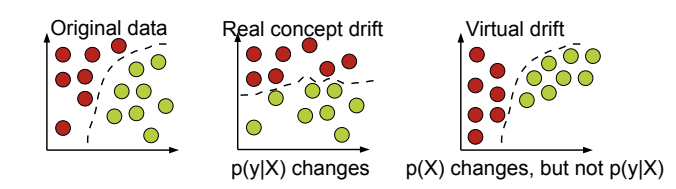
\includegraphics[width=1\textwidth]{my_images/drift_types.png}
    \caption{Types of concept drift. Source:~\cite{drift_adaptation_survey}.}\label{fig:concept_drift_types}
\end{figure}

Although real concept drift is formally defined by changes in $ p(y \mid X) $,
in practice, such changes may be accompanied by observable shifts in the
marginal input distribution $ p(X) $, particularly when certain input regions
become more prevalent or undergo structural changes. However, changes in $ p(X)
$ alone do not guarantee concept drift, as the conditional relationship $ p(y
    \mid X) $ may remain unchanged. Nevertheless, analyzing how $ p(X) $ evolves
over time can offer indirect clues about the presence or potential causes of
concept drift, especially in situations where true labels are unavailable.

In addition to classifying concept drift based on its effect on the data
distribution (i.e., real vs.\ virtual drift), it is also important to consider
the \textit{temporal dynamics} through which drift unfolds. Based on the
taxonomy introduced by Gama et al.~\cite{drift_adaptation_survey}, the temporal
characteristics of concept drift can be categorized as follows:

\begin{itemize}
    \item \textbf{Abrupt drift}: A sudden and immediate change in the joint
          distribution, where the new concept replaces the old one almost
          instantaneously.

    \item \textbf{Incremental drift}: A gradual transition in which the old
          concept is progressively replaced by the new one, potentially passing
          through a continuum of intermediate states.

    \item \textbf{Gradual drift}: A process where both old and new concepts
          coexist for a period, with the probability of observing the new concept
          increasing over time.

    \item \textbf{Recurring drift}: A reappearance of previously
          observed concepts, typically in a periodic or seasonal manner, indicating
          temporal regularity in the drift process.
\end{itemize}

\begin{figure}[H]
    \centering
    \includegraphics[width=1\textwidth]{my_images/drift_temporal_evolution.png}
    \caption{Temporal characterization of concept drift. Source:~\cite{drift_adaptation_survey}.}\label{fig:concept_drift_characterization}
\end{figure}

\subsection*{Drift Detection}\label{subsec:drift_detection}
Concept drift detection identifies changes in the statistical properties of
data streams that affect model performance. A typical framework consists of
four main stages~\cite{learning_under_concept_drift}:

\begin{enumerate}
    \item \textbf{Data Retrieval}: Organizes incoming data into chunks
          suitable for analysis.
    \item \textbf{Data Modeling (Optional)}: Transforms or reduces the data
          for efficiency or interpretability.
    \item \textbf{Test Statistic Computation}: Quantifies differences between
          past and current data or model performance.
    \item \textbf{Hypothesis Testing}: Determines whether detected differences
          are statistically significant.
\end{enumerate}

These stages are common across most detection algorithms and support flexible
implementation across streaming scenarios.

Drift detection algorithms can be broadly categorized into three groups based
on the nature of their test statistics.

\textbf{Error-Rate-Based Methods} monitor the performance of a predictive model.
A significant increase in error rate suggests concept drift.
Notable algorithms include:

\begin{itemize}
    \item \emph{DDM} (Drift Detection Method)~\cite{ddm}: Detects concept drift
          by monitoring the classification error rate and triggering a warning or drift s
          ignal when it statistically deviates from its historical minimum.

    \item \emph{EDDM}~\cite{eddm}: Extends DDM by analyzing the distance between
          consecutive errors, improving sensitivity to gradual and progressive drifts.

    \item \emph{ADWIN}~\cite{adwin}: Uses a variable-length sliding window and
          detects drift by statistically comparing averages in two subwindows, allowing
          automatic adaptation to both abrupt and gradual changes.
\end{itemize}

\textbf{Distribution-Based Methods} compare statistical properties of data distributions directly,
often in an unsupervised setting.

\begin{itemize}
    \item \emph{LSDD}~\cite{lsdd}: Uses a kernel-based method to measure the difference
          between distributions.
    \item \emph{ITA}~\cite{ita} (Information-Theoretic Approach): Relies on entropy and divergence
          measures to detect distributional changes.
    \item \emph{SyncStream}~\cite{syncstream}: Captures synchronized structural changes in multidimensional streams.
\end{itemize}

\textbf{Ensemble and Multi-Test Methods} use multiple statistical tests or detectors in parallel or
hierarchically to improve robustness and adaptivity.

\begin{itemize}
    \item \emph{JIT} (Just-in-Time Drift Detection)~\cite{jit}: Tests various feature combinations
          for localized drift detection.
    \item \emph{HHT} (Hierarchical Hypothesis Testing)~\cite{hht}: Combines quick detection with
          secondary validation to reduce false alarms.
    \item \emph{e-Detector}~\cite{e_detector}: Leverages an ensemble of heterogeneous detectors to
          balance early detection and accuracy.
\end{itemize}

Each category addresses different aspects of the drift detection problem.
Error-rate-based methods are tightly coupled with the model but rely on labeled
data. Distribution-based methods are model-agnostic and can work without
labels, while ensemble and hierarchical approaches aim to improve detection
reliability under varying conditions.

\subsection*{Drift Adaptation}\label{subsec:drift_adaption}

Concept drift adaptation refers to the broad set of techniques designed to
maintain predictive performance in the presence of changing data distributions.
This field is commonly referred to as \emph{Adaptive Learning}.

Gama et al.~\cite{drift_adaptation_survey} classify adaptation strategies into
two primary categories:

\begin{enumerate}
    \item \textbf{Blind methods}: These methods adapt the model continuously or
          periodically, without relying on explicit drift detection mechanisms.
          They are typically simpler and more responsive but may incur unnecessary
          updates when no drift has occurred.
    \item \textbf{Informed methods}: These approaches rely on the output of drift
          detectors to guide the adaptation process. By updating the model only when drift
          is detected, they aim to achieve more efficient and targeted adaptation.
\end{enumerate}

Another perspective proposed by Lu et al.~\cite{learning_under_concept_drift}
focuses on how the model is updated:

\begin{itemize}
    \item \textbf{Simple retraining}: Upon detection of concept drift, the
          current model is discarded and a new one is trained using the most recent
          data. A sliding or adaptive window is often used to select relevant training
          samples.
    \item \textbf{Model adjusting}: Instead of retraining the entire model,
          only affected parts are incrementally updated. This approach is particularly
          effective for handling localized or gradual drift, and is generally more
          efficient.
    \item \textbf{Ensemble retraining}: Rather than relying on a single model,
          ensemble methods maintain a pool of base classifiers. Adaptation is achieved
          by updating, weighting, replacing, or adding classifiers in response to drift,
          making them especially well-suited for handling recurring or complex drifts.
\end{itemize}

The effectiveness of drift adaptation methods depends on the characteristics of
the data stream, such as the type and frequency of drift. A well-designed
adaptive system often combines both detection and adaptation mechanisms to
ensure timely and efficient responses to changes in data distribution.

\subsection*{Drift Explainability}\label{subsec:drift_explainability}

Drift explainability focuses on understanding the causes and nature of changes
in data distributions that affect machine learning models. While detecting
drift is important, it is equally critical to explain why and how drift occurs.
This understanding provides valuable insights into the data evolution and
informs decisions about retraining and maintenance.

There are several techniques for explaining drift, each aiming to reveal how
data shifts influence model behavior. One common approach involves identifying
which features have changed significantly over time and assessing how these
changes impact the model's predictions. For example, \textbf{feature importance
    analysis}~\cite{feture_importance_for_drift_explainabilty} can be used to
compare a model $ f_{\text{ref}} $ trained on reference data $ D_P =
    \{(\mathbf{x}_i, y_i)\}_{i=1}^n \sim P $, where $ P $ is the reference data
distribution and $ n $ is the number of reference samples, with a model $
    f_{\text{prod}} $ trained on production data $ D_Q = \{(\mathbf{x}_j,
    y_j)\}_{j=1}^m \sim Q $, where $ Q $ is the production data distribution and $
    m $ is the number of production samples. Let $ \phi_i^{\text{ref}} $ and $
    \phi_i^{\text{prod}} $ denote the importance of feature $ i $ in the respective
models. A large shift
\begin{equation}
    \Delta \phi_i = \left| \phi_i^{\text{ref}} - \phi_i^{\text{prod}} \right|
\end{equation}
may indicate that feature $ i $ has changed its predictive relationship with the target.

Another powerful approach to drift explainability formulates the detection of
distributional shift as a binary classification problem between the reference
dataset $D_P$ and the production dataset $D_Q$. This method, known as a
\textbf{Classifier Two-Sample Test
    (C2ST)}~\cite{revisiting_two_sample_classifier}, labels samples from $P$ with
class 0 and samples from $Q$ with class 1, and trains a binary classifier $f:
    \mathcal{X} \rightarrow \{0, 1\}$ to distinguish between them.

If the null hypothesis $H_0: P = Q$ holds, then the classification accuracy of
$f$ on a held-out validation set $D_{\text{test}}$ should remain close to
chance level, i.e., $\text{Acc}(f) \approx 0.5$. The test statistic is given
by:
\begin{equation}
    \text{C2ST}(f) = \frac{1}{|D_{\text{test}}|} \sum_{(\mathbf{x}, y) \in D_{\text{test}}} \mathds{1} \{f(\mathbf{x}) = y\}.
\end{equation}
A significant deviation from $0.5$ suggests that $P \neq Q$, indicating distributional drift.

Beyond detection, C2STs offer an interpretable means to explain drift by
examining the feature importances of the trained classifier. This technique
highlights which features $x_i$ contribute most to $f(\mathbf{x})$, and hence
to the difference between $P$ and $Q$.

Understanding the factors behind drift is essential for effective model
management. Without explainability, decisions about retraining may be based on
guesswork, potentially leading to unnecessary updates or degraded performance.
Drift explainability ensures that model updates are both necessary and
well-targeted, guided by principled statistical and model-based insights.
\chapter{Problem formulation}\label{ch:problem_formulation}

\section{Streaming Clustering}\label{sec:prob_streaming_clustering}
A \textit{data stream} is a potentially infinite sequence of multi-dimensional
data points:
\begin{equation}
    \chi = \{x^t\}_{t=1}^{\infty}, \quad x^t \in \mathbb{R}^n
\end{equation}
where $x^t$ denotes the $n$-dimensional observation received at timestamp $t$.
Due to the unbounded nature of data streams and limited memory or computation
constraints, traditional batch clustering methods are not applicable in this
setting.

The goal of streaming clustering is to partition the incoming data points into
groups in a timely and resource-efficient manner. At any given time $t$, a
clustering algorithm processes the stream incrementally and produces a
clustering result:
\begin{equation}
    C^t = \{c_1^t, c_2^t, \dots, c_{k^t}^t\}
\end{equation}
where:
\begin{itemize}
    \item $C^t$ denotes the clustering obtained at time $t$,
    \item $k^t$ is the number of clusters at time $t$,
    \item $c_i^t$ is the $i$-th cluster at time $t$, defined as a subset of data
          points observed up to time $t$.
\end{itemize}

Streaming clustering methods must satisfy the following constraints:

\begin{enumerate}
    \item \textbf{Incrementality:} The algorithm must be able to update the clustering
          with each new incoming data point or small batch, without access to the full
          historical data.

    \item \textbf{Bounded Memory:} The algorithm must operate within limited memory,
          often without storing all previous data points.

    \item \textbf{Computational Efficiency:} The algorithm must produce clustering
          updates within tight time constraints to maintain real-time responsiveness.

    \item \textbf{Adaptability:} The algorithm should be capable of handling non-stationary
          data distributions, as the characteristics of the stream may change over time.
\end{enumerate}

At each time step, the algorithm processes new data and outputs an updated
clustering $C^t$. The clustering may change significantly over time due to
drift, noise, or the arrival of new patterns in the stream.

\section{Tracking Clusters}\label{sec:prob_tracking_clusters}
In non-stationary data streams, clustering structures evolve over time due to
changes in the underlying data distribution. Consequently, the clustering model
$C^t$ at time $t$ may differ substantially from $C^\tau$ at a later time $\tau
    > t$. To analyze such dynamics, it is essential to model and track how
individual clusters change across time.

Given a sequence of clustering models $\{C^0, C^1, \dots, C^T\}$ over time,
where each $C^t = \{c_1^t, \dots, c_{k_t}^t\}$ represents a set of clusters at
time $t$, the goal is to identify and categorize transitions between clusters
over time.

As discussed by Oliveira et Gama~\cite{mec}, clusters may undergo several types
of transitions:

\begin{itemize}
    \item \textbf{Appearance}: A new cluster is formed that did not exist previously.
    \item \textbf{Disappearance}: A previously existing cluster ceases to exist.
    \item \textbf{Split}: A single cluster divides into multiple clusters.
    \item \textbf{Merge}: Multiple clusters combine into a single cluster.
    \item \textbf{Survival}: A cluster remains relatively unchanged over time.
\end{itemize}

To formally define cluster transitions, it is necessary to introduce the notion
of \textbf{overlap} between clusters at different timestamps. Given a cluster $
    c_i^t \in C^t $ and a cluster $ c_j^\tau \in C^\tau $, with $ t < \tau $, these
clusters are said to \emph{overlap}, denoted as
\begin{equation}
    c_i^t \circledast c_j^\tau,
\end{equation}
if they exhibit a non-negligible intersection, as determined by the underlying
cluster representation. The specific definition of overlap depends on the chosen
cluster model. Common examples include:

\begin{itemize}
    \item \textbf{Enumeration-based Representation:}
          \begin{equation}
              c_i^t \circledast c_j^\tau \iff \exists x \in \mathbb{R}^n \text{ such that } x \in c_i^t \land x \in c_j^\tau,
          \end{equation}
          indicating that the two clusters share at least one common data point.

    \item \textbf{Spherical Model Representation:}
          \begin{equation}
              c_i^t \circledast c_j^\tau \iff d(\vec{\mu}_i^t, \vec{\mu}_j^\tau) \leq r_i^t + r_j^\tau,
          \end{equation}
          where $ \vec{\mu}_i^t $ and $ \vec{\mu}_j^\tau $ denote the centroids of
          clusters $ c_i^t $ and $ c_j^\tau $, respectively, $ r_i^t $ and $ r_j^\tau $
          are their radii, and $ d(\cdot, \cdot) $ is the Euclidean distance.
\end{itemize}

The following table summarizes the formal definitions of typical cluster
transitions based on the concept of overlap:

\begin{table}[H]
    \centering
    {\small
        \begin{tabular}{|l|c|p{9cm}|}
            \hline
            \textbf{Transition} & \textbf{Notation}                                 & \textbf{Formal Definition}                                                                            \\
            \hline
            Appearance          & $\emptyset \rightarrow c_j^\tau$                  &
            $\nexists c_i^t \in C^t: c_i^t \circledast c_j^{\tau}$                                                                                                                          \\
            \hline
            Disappearance       & $c_i^t \rightarrow \emptyset$                     & $\nexists c_j^{\tau} \in C^{\tau}: c_i^t \circledast c_j^{\tau}$                                      \\
            \hline
            Split               & $c_i^t \rightarrow \{c_1^\tau, \dots, c_v^\tau\}$ & $\exists\, 1 \leq j \leq v: c_i^t \circledast c_j^\tau \land \dots \land c_i^t \circledast c_v^\tau $ \\
            \hline
            Merge               & $\{c_1^t, \dots, c_u^t\} \rightarrow c_j^\tau$    & $\exists\, 1 \leq i \leq u: c_i^t \circledast c_j^\tau \land \dots \land c_u^t \circledast c_j^\tau $ \\
            \hline
            Survival            & $c_i^t \rightarrow c_j^\tau$                      & $c_i^t \circledast c_j^\tau \land
                \nexists\, c_u^t \in C^t \setminus \{c_i^t\}: c_u^t \circledast c_j^\tau \land
            \nexists\, c_v^\tau \in C^\tau \setminus \{c_j^\tau\}: c_i^t \circledast c_v^\tau$                                                                                              \\
            \hline
        \end{tabular}
    }
    \caption{Formal definitions of cluster transitions}
    \label{table:cluster_transitions}
\end{table}

In contrast to the external transitions described above, which involve
structural changes between distinct clusters over time, \textbf{internal
    transitions} refer to the transformations that occur \emph{within} a single
surviving cluster. These transitions are analyzed only when a cluster persists
across time (i.e., it undergoes a \emph{survival} transition), and they
characterize the evolution of the cluster's internal properties.

Internal transitions typically involve comparisons of specific characteristics
of a cluster between time steps, such as:

\begin{itemize}
    \item \textbf{Expansion or Shrinkage}: Changes in the cardinality (number of
          elements) or spatial extent of a cluster, indicating that the cluster has
          grown or contracted.
    \item \textbf{Density Variation}: Alterations in the density of a cluster,
          often defined in terms of the number of points per unit volume, which may
          suggest dispersion or compaction of the cluster.
    \item \textbf{Centroid Shift}: Movement of the cluster centroid over time,
          reflecting a displacement in the central location of the cluster within the
          feature space.
\end{itemize}

Although internal transitions provide additional insight into the temporal
dynamics of clusters, they are not explicitly addressed in this thesis. The
primary focus is on external transitions, which are more directly related to
the structural evolution of the clustering model. Nevertheless, internal
transitions can be readily inferred by examining the state of a surviving
cluster before and after a time step, allowing for indirect analysis when
needed.

Tracking clusters in dynamic streaming environments presents several key
challenges. One of the foremost difficulties is dealing with concept drift and
evolution, where the underlying data distribution may shift gradually or
abruptly, causing clusters to move, emerge, disappear, merge, or split in
complex and unpredictable ways. The presence of noise and outliers further
complicates the problem by potentially masking genuine cluster transitions or
generating false alarms. Ambiguities often arise when clusters overlap or lie
in close proximity, making it challenging to precisely define cluster
correspondences and detect transitions accurately. Finally, the absence of
ground truth labels in streaming contexts makes it difficult to evaluate the
correctness of detected transitions and adapt algorithms to evolving cluster
structures.

\section{Dynamic Clustering}\label{sec:dynamic_clustering}

Dynamic clustering aims to provide a holistic framework for understanding and
responding to the evolution of data distributions in non-stationary
environments. By combining streaming clustering with temporal cluster tracking,
it enables both real-time analysis and retrospective insight into how clusters
emerge, change, and disappear over time.

The objective is not only to cluster incoming data efficiently, but also to
interpret and explain the structural changes in the data. This is particularly
valuable in applications where understanding data dynamics is as important as
making accurate predictions or decisions.

Dynamic clustering supports a range of analytical goals, including:

\begin{itemize}
    \item \textbf{Drift Explainability:} By analyzing the history and transformation of
          clusters, one can identify when and how concept drift occurs, and potentially
          relate it to changes in user behavior, system state, or external conditions.

    \item \textbf{Concept Monitoring and Lifecycle Analysis:} Tracking clusters over time
          provides a basis for monitoring the emergence, evolution, and retirement of
          underlying concepts or patterns in the data.

    \item \textbf{Anomaly and Event Detection:} Sudden transitions—such as abrupt merges,
          splits, or disappearances—can signal significant events or anomalies in the data stream,
          such as system faults or behavioral shifts.

    \item \textbf{Interpretability and Visualization:} Visualizing cluster evolution as
          trajectories, trees, or timelines helps domain experts make sense of complex temporal
          dynamics in an intuitive manner.
\end{itemize}

By treating clustering as a dynamic process rather than a static task, this
framework enables richer, more actionable insights in data-driven systems that
operate under change.
\chapter{State of the Art}\label{ch:state_of_the_art}

\section{Streaming Clustering Algorithms}\label{sec:streaming_clustering_algorithms}

Streaming clustering algorithms are designed to handle continuously arriving
data streams efficiently while adapting to changes in the underlying data
distribution. Unlike traditional batch clustering methods, streaming clustering
must operate under constraints such as limited memory, the impossibility of
revisiting old data, and the need for real-time processing. As discussed by
Zubaroglu et Atalay~\cite{streaming_clustering_review}, the main categories of
streaming clustering algorithms are: hierarchical, partitioning-based,
density-based, grid-based, and model-based methods.

\textbf{Hierarchical streaming clustering} algorithms produce nested clusters organized
in a tree-like structure called a dendrogram, which offers a rich and interpretable
summary of data relationships. These methods are divided into \textit{agglomerative} (bottom-up)
and \textit{divisive} (top-down) approaches. Agglomerative algorithms start by treating
each data point as a separate cluster and iteratively merge clusters based on similarity,
whereas divisive algorithms begin with all data points in a single cluster and recursively
split them. Although hierarchical methods provide detailed cluster structures, their high
computational complexity and sensitivity to noise and outliers make them less suitable for
high-velocity data streams. Examples include \textsc{BIRCH}~\cite{birch} and
\textsc{HUE-Stream}~\cite{hue_stream}.

\textbf{Partitioning-based streaming algorithms} divide data into a predefined number of clusters
by optimizing an objective function, commonly based on distance measures to cluster centroids. They
maintain compact data summaries such as micro-clusters or cluster feature vectors to efficiently update
clusters incrementally. These algorithms are computationally efficient and easy to implement; however,
they generally require prior knowledge of the number of clusters and tend to identify only spherical
or convex clusters. Notable examples include \textsc{CluStream}~\cite{clustream} and
\textsc{StreamKM++}~\cite{stream_km_plus_plus}.

\textbf{Density-based methods} identify clusters as regions of high data density separated by
regions of low density. In streaming contexts, they maintain summaries of dense micro-clusters
that evolve over time, allowing them to discover arbitrarily shaped clusters and automatically
detect the number of clusters. These methods also demonstrate robustness to noise and outliers.
However, they typically require multiple user-defined parameters and can struggle when clusters
have varying densities. Representative algorithms include \textsc{DenStream}~\cite{denstream}
and \textsc{D-Stream}~\cite{d_stream}.

\textbf{Grid-based streaming clustering} approaches partition the data space into a finite number
of cells or grids and cluster these cells based on their density or other summary statistics. This
discretization allows for fast updates and scalable clustering as runtime depends primarily on the
number of cells rather than the number of data points. Grid-based methods are naturally robust to
noise and can detect clusters of arbitrary shapes; however, their performance decreases in high-dimensional
spaces due to the exponential growth of grid cells. Additionally, the choice of grid granularity heavily
influences clustering results. Examples include \textsc{MR-Stream}~\cite{mr_stream}
and \textsc{CLIQUE}~\cite{clique}.

\textbf{Model-based streaming clustering algorithms} assume that data are generated from a mixture of
underlying probability distributions and aim to identify these models incrementally. These approaches
offer principled frameworks with strong noise robustness and can incorporate prior knowledge through
model selection. However, their effectiveness depends on the appropriateness of the selected model,
and they often involve complex parameter estimation procedures. Algorithms in this category include
\textsc{COBWEB}~\cite{cobweb} and \textsc{CluDistream}~\cite{cludistream}.

\begin{table}[H]
    \centering

    \begin{tabular}{|l|p{6cm}|p{6cm}|}
        \hline
        \textbf{Category} & \textbf{Advantages}                                                & \textbf{Disadvantages}                                                 \\
        \hline
        Hierarchical      & Provides detailed cluster hierarchy and interpretable dendrograms  & High computational complexity; sensitive to noise and outliers         \\
        Partitioning      & Efficient and easy to implement; suitable for large-scale data     & Requires predefined number of clusters; limited to spherical clusters  \\
        Density-Based     & Detects arbitrary shapes; robust to noise; adaptive cluster number & Sensitive to parameter settings; struggles with multi-density clusters \\
        Grid-Based        & Fast updates; scalable; noise robust; detects arbitrary shapes     & Degrades in high dimensions; depends on grid size choice               \\
        Model-Based       & Robust to noise; interpretable probabilistic framework             & Depends heavily on model selection; computationally intensive          \\
        \hline
    \end{tabular}
    \caption{Comparison of Streaming Clustering Approaches}
    \label{table:streaming-clustering-comparison}
\end{table}

Each category offers distinct advantages and limitations, summarized in Table
~\ref{table:streaming-clustering-comparison}. Despite significant progress,
several challenges remain in streaming clustering research, such as
automatically adapting to concept drift, handling evolving cluster structures,
and providing explanations for cluster evolution. These gaps motivate the
development of dynamic clustering frameworks that combine streaming processing
with cluster tracking and evolution analysis, enabling advanced applications
including drift explainability.

The following subsection introduces CluStream, a widely adopted framework for
dynamic clustering that serves as a foundational component in numerous existing
systems. Owing to its modular architecture and demonstrated practical
effectiveness, CluStream has been extensively implemented and integrated into
various real-time data stream clustering solutions.

\subsection{CluStream}\label{subsec:clustream}

CluStream~\cite{clustream} is a widely adopted framework designed for
clustering evolving data streams. It operates on a two-phase architecture that
separates online data summarization from offline cluster analysis, balancing
real-time efficiency with analytical depth.

\paragraph{Online Micro-Clustering} The online phase processes incoming data in real time, incrementally
summarizing the stream into a set of \textit{micro-clusters}. Each
micro-cluster is a temporal summary of a group of data points and is defined
using a variant of the Clustering Feature (CF) vector:

\begin{equation}
    \text{MC} = \left( \vec{LS}, SS, \vec{TS}, n \right)
\end{equation}

where:
\begin{itemize}
    \item $\vec{LS} = \sum_{i=1}^{n} \vec{x}_i$ is the linear sum of $n$ $d$-dimensional data points,
    \item $\vec{SS} = \sum_{i=1}^{n} \vec{x}_i \cdot \vec{x}_i$ is the sum of squares,
    \item $\vec{TS} = \sum_{i=1}^{n} t_i$ is the sum of timestamps,
    \item $n$ is the number of points contained in the micro-cluster.
\end{itemize}

From these quantities, the following statistics can be derived:
\begin{itemize}
    \item \textbf{Centroid}:
          \begin{equation}
              \vec{\mu} = \frac{\vec{LS}}{n}
          \end{equation}
    \item \textbf{Standard Deviation}:
          \begin{equation}
              \sigma = \sqrt{ \frac{\vec{SS}}{n} - \left( \frac{\vec{LS}}{n} \right)^2 }
          \end{equation}
\end{itemize}

Incoming data points are assigned to the nearest micro-cluster if the distance
to its centroid is below a threshold, often proportional to the cluster's
standard deviation. If the point does not fit within any existing
micro-cluster, a new one is created. To maintain a fixed budget of
micro-clusters (denoted by $q$), the algorithm either merges the two closest
micro-clusters or removes the least recently updated one.

When two micro-clusters $MC_1$ and $MC_2$ are merged, the resulting
micro-cluster is defined as:

\begin{align}
    \vec{LS}^{\text{new}} & = \vec{LS}^{(1)} + \vec{LS}^{(2)} \\
    \vec{SS}^{\text{new}} & = \vec{SS}^{(1)} + \vec{SS}^{(2)} \\
    \vec{TS}^{\text{new}} & = \vec{TS}^{(1)} + \vec{TS}^{(2)} \\
    n^{\text{new}}        & = n^{(1)} + n^{(2)}
\end{align}

\paragraph{Pyramidal Time Frame} To support temporal analysis, CluStream maintains snapshots of the current set
of micro-clusters at multiple temporal granularities. Snapshots are stored at
exponentially spaced intervals (e.g., 1, 2, 4, 8, $\dots$ time units), forming
a pyramidal time frame that allows efficient reconstruction of historical
cluster states with logarithmic storage complexity.

\paragraph{Offline Macro-Clustering} At user-specified intervals or upon query, the offline phase performs
macro-clustering using the current or historical micro-cluster summaries. This
typically involves applying a conventional clustering algorithm (e.g., weighted
$k$-Means) to the centroids of the micro-clusters, where each centroid is
weighted by the number of data points $n$ it represents. This enables efficient
clustering over a condensed, noise-reduced representation of the data stream.

This modular architecture enables CluStream to efficiently handle high-speed
data streams while supporting accurate and scalable offline analysis.

\section{Tracking Clusters Algorithms}\label{sec:tracking_clusters_algorithms}

The challenge of tracking evolving clustering structures in non-stationary data
streams has garnered increasing attention, leading to the development of
numerous methods designed to capture and explain transitions such as the
emergence, disappearance, splitting, merging, and persistence of clusters over
time. This section reviews the key methodologies corresponding to the
transition types outlined in Section~\ref{sec:prob_tracking_clusters},
organizing them according to the algorithmic paradigms they follow, as also
done by Atif et al.~\cite{tracking_review}.

\textbf{Self-Organizing Maps (SOMs)} change tracking and it is build on the idea of
learning low-dimensional topological representations of high-dimensional temporal data.

Denny and Squire~\cite{som_tracking} proposed a method where \textsc{SOMs} are
trained sequentially on snapshots $D_{t_i}$ and $D_{t_{i+1}}$, with cluster
assignments determined using $k$-means. Although the method can track survival
and shifts in centroid position, it fails to reliably detect emerging or
disappearing clusters due to static initialization and dependency on prior
topology.

To address this, \textsc{ReDSOM}~\cite{redsom_tracking} was developed to
compare density distributions and centroid shifts between successive SOMs. It
supports identification of transitions such as:

\begin{itemize}
    \item Disappearance: Regions with reduced density and unmapped data.

    \item Appearance: Newly populated map regions.

    \item Enlargement/Contraction: Changes in the spread of mapped data.
\end{itemize}

However, SOM-based methods may struggle with overlapping or nested clusters due
to their grid-constrained topology.

\textbf{Heuristic and Graph-Based Algorithms} are distinct family of algorithms focuses
on tracking structural transitions through direct comparison of clustering results at
successive time points.

\textsc{MONIC} (Spiliopoulou et al.~\cite{monic}) is a seminal heuristic framework that uses an overlap
matrix $O_{ij}$ between clusters $X_i$ at $t$ and $Y_j$ at $\tau > t$.
The overlap matrix is defined as:
\begin{equation}
    O_{ij} = \frac{|X_i \cap Y_j|}{|X_i|}, \quad i = 1, \ldots, k_1, \quad j = 1, \ldots, k_2.
\end{equation}

Transitions are categorized as:
\begin{itemize}
    \item Appearance: $\nexists X_i: O_{ij} > \theta$

    \item Disappearance: $\nexists Y_j: O_{ij} > \theta$

    \item Merge/Split: Multiple significant overlaps across time

    \item Survival: One-to-one high overlap

    \item Internal Transition: Changes in size or centroid within a surviving cluster
\end{itemize}

This directly aligns with the transition framework from
Table~\ref{table:cluster_transitions} but requires pre-defined overlap
thresholds and can manage only clusters with enumeration representation.

\textsc{MONIC+} (Ntoutsi et al.~\cite{monic_plus}) generalizes the overlap function by incorporating cluster-type-specific
definitions. MONIC+ supports three distinct types of clusters based on how they are represented and formed:
\begin{itemize}
    \item Type A Clusters (Geometric Clusters): Discovered in a dataset-independent
          metric space, these clusters are defined by their geometric properties (e.g.,
          spheres in k-means). Cluster transitions are observed as geometric
          transformations over time.
          \begin{equation}
              \text{overlap}(X,Y) = \frac{\text{area}(X \cap Y)}{\text{area}(X)}
          \end{equation}
    \item Type B1 Clusters (Set-based Clusters): These clusters are defined extensionally
          as sets of data records without relying on a fixed metric space. Algorithms
          like hierarchical clustering fall under this category. The data-dependent
          nature of the metric space means that adding a new point can affect cluster
          boundaries indirectly.
          \begin{equation}
              \text{overlap}(X,Y) = \frac{\sum_{a \in X \cap Y} \text{age}(a, t_j)}{\sum_{a \in X} \text{age}(a, t_j)}
          \end{equation}
    \item Type B2 Clusters (Distribution-based Clusters): Clusters here are defined
          intensionally as statistical distributions. A cluster $X$ is characterized by
          its cardinality $\text{card}(X)$, mean $\mu(X)$, and standard deviation
          $\sigma(X)$. The Expectation-Maximization (EM) algorithm is a typical example.
          \begin{equation}
              \text{overlap}(X, Y) =
              \begin{cases}
                  1 - \dfrac{|\mu(X) - \mu(Y)|}{\sigma(X)} & \text{if } |\mu(X) - \mu(Y)| \leq \sigma(X) \\
                  0                                        & \text{otherwise}
              \end{cases}
          \end{equation}
\end{itemize}

\textsc{MClusT} (Oliveira and Gama~\cite{mclust}) extends MONIC by representing transitions via a
bipartite graph weighted by conditional probabilities between clusters over time.
This probabilistic approach refines the detection of transitions and facilitates intuitive
visualization of merges and splits.
\begin{equation}
    \text{weight}(C_u, C_m) = P(X \in C_u(t_j) \mid X \in C_m(t_i)) =
    \frac{\sum_{m=1}^p P(X \in C_m(t_i) \cap C_u(t_j))}{\sum_{m=1}^p P(X \in C_m(t_i))}
\end{equation}

\textsc{MEC} (Oliveira and Gama~\cite{mec}) introduces an alternative bipartite-graph-based visualization
tool, emphasizing structural comparison of clusters at static intervals. It uses conditional
probability edges to identify transitions similar to MONIC, reinforcing the notion of transition
tracking via inter-temporal matching.

\textbf{Evolutionary Clustering} foundamental concept is to balance temporal smoothness
with clustering accuracy at each time point. Chakrabarti et al.~\cite{evolutionary_clustering}
introduced the evolutionary clustering framework, in which the objective is to compute clustering
solutions $C_t$ for each time step $t$ that are both representative of the current data snapshot
and consistent with past clusterings. The trade-off is formalized as:
\begin{equation}
    \sum_{t=1}^T sq(C_t, M_t) - cp \sum_{t=2}^T hc(C_{t-1}, C_t)
\end{equation}

Here, $sq$ represents snapshot quality, $hc$ denotes history cost, and $cp$ is
a change penalty. Transitions such as \textit{survival} and \textit{small
    structural shifts} are naturally captured through low history cost values,
while abrupt transitions (e.g., \textit{split}, \textit{merge}, or
\textit{appearance}) incur higher costs unless strongly justified by the
snapshot quality.

Chi et al.~\cite{spectral_evolutionary_clustering} extended this approach via
evolutionary spectral clustering, optimizing a cost of the form:
\begin{equation}
    C_{total} = \alpha C_{temporal} + (1-\alpha)C_{snapshot}
\end{equation}

Zhang et al.~\cite{density_evolutionary_clustering} adapted the framework for
density-based clustering (evolutionary DBSCAN) using a similar cost function.
This variant directly supports transitions like appearance and disappearance of
clusters by relying on density thresholds, but it requires parameter tuning
that limits scalability.

Xu et al.~\cite{adaptive_evolutionary_clustering} introduced an adaptive
evolutionary framework that updates proximity matrices recursively. This
supports continuous tracking of survival, gradual merges, or splits, but the
approach is computationally intensive and NP-hard in general.

\section{Dynamic Clustering Algorithms}\label{sec:dynamic_clustering_algorithms}

In recent years, several works have been proposed to address the dynamic
clustering problem by integrating streaming clustering and cluster evolution
tracking into unified frameworks. These approaches aim not only to detect
meaningful cluster structures in evolving data streams but also to monitor how
these clusters evolve over time—capturing events such as survival, absorption,
split, disappearance, and emergence. The primary challenges lie in efficiently
processing high-velocity data, detecting structural changes in the clustering,
and distinguishing between transient and persistent transitions.

Namitha et al.~\cite{namitha_dynamic_clustering_1} proposed a method that
combines CluStream with an estimation of the number of macro-clusters using the
Ordered Multiple Runs of k-Means (OMRk)~\cite{omrk} algorithm. A Simplified
Silhouette index is used as the relative clustering validity criterion.
Macro-clustering is performed over fixed-size windows. Their model explicitly
considers external transitions such as \textit{survival}, \textit{absorption},
and \textit{split}:

\begin{itemize}
    \item \textbf{Survival:} A cluster $X \in C_i$ is said to have survived as $Y \in C_j$ if:
          \begin{enumerate}
              \item The distance between the centroids of $X$ and $Y$ is less than the radius of
                    $X$.
              \item The ratio of the radii of $Y$ and $X$ lies between 0.75 and 1.25.
          \end{enumerate}

    \item \textbf{Absorption:} A cluster $X \in C_i$ is said to be absorbed by $Y \in C_j$ if:
          \begin{enumerate}
              \item The distance between the centroids of $X$ and $Y$ is less than the radius of
                    $Y$.
              \item The radius of $X$ is less than the distance between their centroids.
          \end{enumerate}

    \item \textbf{Split:} A cluster $X \in C_i$ is said to split into clusters $Y_1, Y_2, \dots$ in $C_j$ if:
          \begin{enumerate}
              \item The centroids of $Y_1, Y_2, \dots$ fall within the radius of $X$.
              \item Their radii are smaller than the radius of $X$.
              \item The ratio of the total number of points in $Y_1, Y_2, \dots$ to the number of
                    points in $X$ is between 0.6 and 1.
          \end{enumerate}
\end{itemize}

Clusters that do not fall into any of these categories are classified as
\textbf{disappeared} (in $C_j$) or \textbf{emerged} (in $C_j$ but not derived
from $C_i$).

In a subsequent work, Namitha et al.~\cite{namitha_dynamic_clustering_2}
proposed replacing the fixed-size window approach with a drift detection
mechanism based on the Page-Hinkley test~\cite{page_hinkley}. For each new data
point, the distance to the nearest cluster is monitored to detect
distributional changes. This approach triggers macro-clustering only when
necessary and explicitly integrates the MONIC algorithm for cluster transition
tracking.

Lima and Sousa introduced CETra (Cluster Evolution Tracker)~\cite{cetra}, an
online cluster tracking framework tailored for disjoint clusters that evolve
gradually. CETra maintains a \textit{referential clustering}
$\zeta_{\text{ref}}^{t_i}$ in memory, used as a basis for comparison with
successive \textit{evolutionary clusterings} $\zeta^{t_j}$:

\begin{itemize}
    \item A clustering remains referential until a significant divergence from subsequent
          clusterings is observed.
    \item This approach allows CETra to distinguish between gradual evolution and
          transient changes.
    \item Both external and internal transitions are considered, enabling a complete
          evolution tracking mechanism.
\end{itemize}

Feng et al.\ proposed OCEAN~\cite{ocean}, a completely online clustering
algorithm based on a grid-partitioning scheme. OCEAN reduces spatial complexity
by:

\begin{itemize}
    \item Maintaining concrete cluster statistics in each grid cell for real-time
          processing.
    \item Employing an adaptive composite windowing strategy that combines current and
          historical data windows, dynamically adjusting their widths.
    \item Supporting multiple clustering scenarios and providing evolution analysis
          through the composite window to improve clustering efficiency.
\end{itemize}

Overall, dynamic clustering methods aim to efficiently and accurately detect
cluster evolution over time. While some rely on summarization techniques and
periodic re-clustering, others emphasize online monitoring and drift detection
to adapt to changes in real time.
\chapter{Method}\label{ch:method}

This chapter presents a novel framework for addressing the dynamic clustering
problem. It begins with the introduction of a new class of transitions that
incorporates the recurrence of specific cluster evolutions over time, enabling
a more realistic modeling of evolving data streams. A new formulation of
overlapping scores is then proposed for both spherical and Gaussian clusters,
allowing for a more precise quantification of cluster overlap. In addition, a
triggering mechanism based on the CluStream micro-clustering algorithm is
introduced to detect significant structural changes in the data. The chapter
concludes with a detailed description of the framework's architecture,
outlining its components and their interactions in supporting adaptive and
interpretable streaming clustering.

\section{Extended Transitions}\label{sec:extended_transitions}

To more accurately capture the dynamic evolution of clusters over time, this
section introduces an extension to the traditional notion of transitions.
Instead of relying solely on pairwise comparisons or aggregate statistics,
transitions are modeled using a structured and interpretable representation. As
described in MEC, one effective approach is to represent transitions between
two clustering results as a \textbf{bipartite graph}. In this graph, each node
represents a cluster at a specific time point, and edges indicate the degree of
overlap between clusters across two consecutive timestamps.

This representation enables a principled framework for identifying and
classifying transition patterns. Each edge encodes a correspondence between
clusters, allowing the system to categorize transitions such as
\emph{survivals}, \emph{splits}, \emph{merges}, \emph{appearances}, and
\emph{disappearances}, based on the edge connectivity patterns. The resulting
graph-based model facilitates a more expressive and insightful analysis of
cluster evolution.

\begin{figure}[H]
    \centering
    \begin{tikzpicture}[
            leftnode/.style={circle, draw=blue!60, fill=blue!5, thick, minimum size=7mm},
            rightnode/.style={circle, draw=orange!60, fill=orange!5, thick, minimum size=7mm},
            font=\sffamily,
            node distance=8mm and 30mm
        ]

        % Time labels
        \node[font=\bfseries] at (0,2) {$t$};
        \node[font=\bfseries] at (4.2,2) {$\tau$};

        % Left nodes (1 to 5)
        \node[leftnode] (n1) at (0,1) {1};
        \node[leftnode] (n2) at (0,0) {2};
        \node[leftnode] (n3) at (0,-1) {3};
        \node[leftnode] (n4) at (0,-2) {4};
        \node[leftnode] (n5) at (0,-3) {5};

        % Right nodes (6 to 10)
        \node[rightnode] (n6) at (4,1) {6};
        \node[rightnode] (n7) at (4,0) {7};
        \node[rightnode] (n8) at (4,-1) {8};
        \node[rightnode] (n9) at (4,-2) {9};
        \node[rightnode] (n10) at (4,-3) {10};

        % Edges
        \draw[->, thick] (n2) -- (n7);
        \draw[->, thick] (n2) -- (n8);
        \draw[->, thick] (n3) -- (n9);
        \draw[->, thick] (n4) -- (n9);
        \draw[->, thick] (n5) -- (n10);

        % Transitions legend centered vertically
        \node[align=left, anchor=center, text width=6cm, draw, rounded corners] (legend) at (8.5,-1) {
            \textbf{Transitions:} \\
            1 disappeared: $1 \rightarrow \emptyset$ \\
            2 splits into 7 and 8: $2 \rightarrow \{7, 8\}$ \\
            3 and 4 merge into 9: $\{3, 4\} \rightarrow 9$ \\
            5 survives as 10: $5 \rightarrow 10$ \\
            6 appeared: $\emptyset \rightarrow 6$
        };

    \end{tikzpicture}
    \caption{Example of transitions from clusters at time $t$ to clusters at time $\tau$.}
    \label{fig:cluster-transitions}
\end{figure}

To support fine-grained tracking and avoid ambiguity in complex transitions,
events such as merges and splits are decomposed into \textbf{atomic
      transitions}. Each atomic transition links a single source cluster to a
destination cluster (or vice versa), enabling a clearer interpretation of
compound transitions.

\begin{figure}[H]
    \centering
    \begin{minipage}{0.55\textwidth}
        \centering
        \begin{tikzpicture}[
                leftnode/.style={circle, draw=blue!60, fill=blue!5, thick, minimum size=7mm},
                rightnode/.style={circle, draw=orange!60, fill=orange!5, thick, minimum size=7mm},
                font=\sffamily,
                node distance=8mm and 30mm
            ]

            % Time labels
            \node[font=\bfseries] at (0,2) {$t$};
            \node[font=\bfseries] at (4.2,2) {$\tau$};

            % Left nodes (1 to 5)
            \node[leftnode] (n1) at (0,1) {1};
            \node[leftnode] (n2) at (0,0) {2};
            \node[leftnode] (n3) at (0,-1) {3};
            \node[leftnode] (n4) at (0,-2) {4};
            \node[leftnode] (n5) at (0,-3) {5};

            % Right nodes (6 to 10)
            \node[rightnode] (n6) at (4,1) {6};
            \node[rightnode] (n7) at (4,0) {7};
            \node[rightnode] (n8) at (4,-1) {8};
            \node[rightnode] (n9) at (4,-2) {9};
            \node[rightnode] (n10) at (4,-3) {10};

            % Edges
            \draw[->, thick] (n2) -- (n7) node[midway, above] {a};
            \draw[->, thick] (n2) -- (n8) node[midway, above] {b};
            \draw[->, thick] (n3) -- (n9) node[midway, above] {c};
            \draw[->, thick] (n4) -- (n9) node[midway, above] {d};
            \draw[->, thick] (n5) -- (n10) node[midway, above] {e};

        \end{tikzpicture}
    \end{minipage}
    \hfill
    \begin{minipage}{0.4\textwidth}
        \centering
        \begin{tabular}{|c|c|c|l|}
            \hline
            \textbf{Edge} & \textbf{From} & \textbf{To} & \textbf{Type} \\
            \hline
            -             & 1             & -           & Disappearance \\
            a             & 2             & 7           & Split         \\
            b             & 2             & 8           & Split         \\
            c             & 3             & 9           & Merge         \\
            d             & 4             & 9           & Merge         \\
            e             & 5             & 10          & Survival      \\
            -             & -             & 6           & Appearance    \\
            \hline
        \end{tabular}
    \end{minipage}
    \caption{Example of atomic cluster transitions between time $t$ and $\tau$.}
    \label{fig:atomic-cluster-transitions}
\end{figure}

The classification of transitions relies on analyzing the degree of
connectivity (i.e., number of incident edges) for each node in the bipartite
graph constructed between clustering results at times $t$ and $\tau$:

\begin{itemize}
      \item \textbf{At time $t$}:
            \begin{itemize}
                  \item A cluster with no outgoing edges is labeled as \emph{disappeared}.
                  \item A cluster with multiple outgoing edges is considered to have undergone a
                        \emph{split}.
            \end{itemize}

      \item \textbf{At time $\tau$}:
            \begin{itemize}
                  \item A cluster with no incoming edges is marked as \emph{newly appeared}.
                  \item A cluster with multiple incoming edges is the result of a \emph{merge}.
            \end{itemize}
\end{itemize}

When a cluster node at either time $t$ or $\tau$ has exactly one connecting
edge, the nature of the transition cannot be inferred directly from the graph
structure alone. In such cases, additional context is needed to disambiguate:

\begin{itemize}
      \item \textbf{From time $t$ to $\tau$}:
            \begin{itemize}
                  \item If the destination cluster has only one incoming edge, the transition is a
                        \emph{survival}.
                  \item If the destination cluster has multiple incoming edges, the source cluster has
                        \emph{merged} with others.
            \end{itemize}

      \item \textbf{From time $\tau$ to $t$}:
            \begin{itemize}
                  \item If the originating cluster has only one outgoing edge, the transition is a
                        \emph{survival}.
                  \item If the originating cluster has multiple outgoing edges, it has \emph{split}.
            \end{itemize}
\end{itemize}

When both nodes involved in a transition have exactly one edge but are each
involved in other connections, the transition is labeled as a
\textbf{mergesplit}, representing a complex reconfiguration that combines
merging and splitting behaviors.

\begin{figure}[H]
    \centering
    \begin{tikzpicture}[
            leftnode/.style={circle, draw=blue!60, fill=blue!5, thick, minimum size=7mm},
            rightnode/.style={circle, draw=orange!60, fill=orange!5, thick, minimum size=7mm},
            font=\sffamily,
            node distance=8mm and 30mm
        ]

        % Time labels
        \node[font=\bfseries] at (0,2) {$t$};
        \node[font=\bfseries] at (4.2,2) {$\tau$};

        % Left nodes
        \node[leftnode] (n1) at (0,1) {1};
        \node[leftnode] (n2) at (0,0) {2};

        % Right nodes
        \node[rightnode] (n6) at (4,1) {6};
        \node[rightnode] (n7) at (4,0) {7};

        % Edges
        \draw[->, thick] (n1) -- (n6) node[midway, above] {a};
        \draw[->, thick] (n1) -- (n7) node[midway, above] {b};
        \draw[->, thick] (n2) -- (n7) node[midway, above] {c};

        % Legend (left)
        \node[align=left, anchor=center, text width=6cm, draw, rounded corners] (legend) at (8.5,0.5) {
            \textbf{Transitions:} \\
            1 splits into 6 and 7: $1 \rightarrow \{6, 7\}$ \\
            1 and 2 merge into 7: $\{1, 2\} \rightarrow 7$
        };

    \end{tikzpicture}

    \vspace{1em}

    % Table below the diagram
    \begin{minipage}{0.8\textwidth}
        \centering
        \begin{tabular}{|c|c|c|l|}
            \hline
            \textbf{Edge} & \textbf{From} & \textbf{To} & \textbf{Transition Type} \\
            \hline
            a             & 1             & 6           & Split                    \\
            b             & 1             & 7           & Mergesplit               \\
            c             & 2             & 7           & Merge                    \\
            \hline
        \end{tabular}
    \end{minipage}
    \caption{Example of a mergesplit transition.}
    \label{fig:cluster-mergesplit}
\end{figure}

While the transitions discussed so far describe short-term structural changes
between consecutive timestamps, long-term dynamics often involve recurring
patterns. To support extended temporal analysis, three additional transition
types are introduced: \textbf{reappearance}, \textbf{remerge}, and
\textbf{resplit}.

\begin{itemize}
      \item \textbf{Reappearance} occurs when a cluster that previously disappeared re-emerges after a delay. To detect this, information about disappeared clusters is retained. If a new cluster in a future timestep significantly overlaps with one of these stored clusters, it is classified as a reappearance rather than a new appearance.

      \item \textbf{Remerge} describes a situation in which a previously merged cluster splits and, at a later point, its components reassemble into a similar structure. The system tracks the identities of the original components, allowing for recognition of this reformation.

      \item \textbf{Resplit} is the converse case, where clusters that previously resulted from a split later recombine. If the new merged cluster shows significant overlap with the original parent cluster, the event is identified as a resplit.
\end{itemize}

By incorporating these extended transition types, the framework enables not
only the detection of immediate structural changes but also the identification
of long-term recurrences. This allows for a more nuanced and temporally aware
analysis of cluster evolution in dynamic environments.

\section{Overlapping Scores Definition}\label{sec:overlapping_scores}
Overlapping scores are used to quantify the degree of similarity or interaction
between two clusters. In dynamic clustering, such scores play a crucial role in
understanding cluster evolution. This section introduces two novel
formulations: one tailored for spherical clusters, and one for Gaussian
clusters with arbitrary covariance structures.

\subsubsection*{Custom Overlapping Score for Spherical Clusters}

For clusters with approximately spherical shapes, the following \textbf{Custom
      Overlapping Score (CustomOS)} is proposed:

\begin{equation}
      \text{CustomOS}(c_1, c_2) = 2^{- \frac{d(\mu_1, \mu_2)}{r_1 + r_2}}
\end{equation}

where:
\begin{itemize}
      \item $ d(\mu_1, \mu_2) $ is the Euclidean distance between the centers of clusters $ c_1 $ and $ c_2 $,
      \item $ r_1 $ and $ r_2 $ represent the respective radii (or characteristic sizes) of the clusters.
\end{itemize}

\textbf{Properties and Interpretation:}
\begin{itemize}
      \item The score is bounded in $ (0, 1] $, where:
            \begin{itemize}
                  \item $ \text{CustomOS} \to 0 $: the clusters are very distant.
                  \item $ \text{CustomOS} = 0.5 $: the clusters are tangent, i.e., $ d(\mu_1, \mu_2) = r_1 + r_2 $.
                  \item $ \text{CustomOS} = 1 $: the clusters are completely overlapped, i.e., $ d(\mu_1, \mu_2) = 0 $.
            \end{itemize}

      \item The score decays exponentially with the normalized inter-cluster distance,
            providing a \textit{scale-invariant} measure of similarity.

      \item The score can be interpreted as a \textbf{probability-like value} quantifying
            the likelihood that two clusters are evolutionarily related. The most uncertain
            case is when the clusters are tangent ($ \text{CustomOS} = 0.5 $), where:
            \begin{itemize}
                  \item $ c_2 $ could be the evolution of $ c_1 $ with a large center shift (i.e., $ d = r_1 + r_2 $),
                  \item or $ c_2 $ could represent a newly formed cluster that emerged near $ c_1 $.
            \end{itemize}

      \item Thanks to these properties, a natural threshold for deciding overlap is $
                  \epsilon = 0.5 $. Scores above this suggest potential continuity or evolution;
            scores below indicate separation.

      \item The score requires only the cluster centers and radii to compute, which makes
            it particularly suitable for \textbf{streaming clustering frameworks} where
            retaining all data points is infeasible. This supports lightweight and
            efficient computation.

      \item Particularly effective in micro-clustering approaches like CluStream, where
            clusters are maintained using summary statistics.
\end{itemize}

\subsubsection*{Effective Overlapping Score for Gaussian Clusters}

Building upon the idea of the \textit{Custom Overlapping Score}, which assumes
spherical symmetry, the \textbf{Effective Overlapping Score (EffectiveOS)}
generalizes the concept to clusters modeled as multivariate Gaussian
distributions. This allows for the consideration of anisotropy and correlated
features by incorporating covariance structure into the overlap estimation.

The \textbf{EffectiveOS} is defined as:

\begin{equation}
      \text{EffectiveOS} = 2^{\frac{-d_M(\mu_1, \mu_2)}{\text{RMSSize}_1 + \text{RMSSize}_2}}
\end{equation}

where $ d_M(\mu_1, \mu_2) $ is the Mahalanobis distance between the cluster
means:

\begin{align}
      d_M(\mu_1, \mu_2) & = \sqrt{(\mu_1 - \mu_2)^\top \Sigma_{12}^{-1} (\mu_1 - \mu_2)} \\
      \Sigma_{12}       & = \frac{\Sigma_1 + \Sigma_2}{2}
\end{align}

The term $ \text{RMSSize}_j $ represents the \textbf{root mean square size} of
cluster $ j $, capturing its generalized radius along principal directions:

\begin{align}
      \text{RMSSize}_j & = \sqrt{\frac{1}{n} \sum_{i=1}^n a_i^2} \\
      a_i              & = \chi^2_\alpha \sqrt{\lambda_i^j}
\end{align}

where:
\begin{itemize}
      \item $ \lambda_i^j $ are the eigenvalues of the covariance matrix $ \Sigma_j $,
            corresponding to the variance along each principal axis of cluster $ j $,
      \item $ \chi^2_\alpha $ is the critical value of the chi-squared distribution at
            confidence level $ \alpha $, scaling the eigenvalues to a desired confidence boundary.
\end{itemize}

\textbf{Properties and Intuition:}
\begin{itemize}
      \item \textbf{Generalization of Spherical Case:} When covariance matrices are multiples
            of the identity, the Mahalanobis distance reduces to the Euclidean distance, and
            RMSSize approximates the radius, thus reducing to the CustomOS formulation.
      \item \textbf{Covariance-aware Distance:} The Mahalanobis distance accounts for
            feature correlation and direction-dependent spread, making it suitable for ellipsoidal clusters.
      \item \textbf{Confidence-aware Scaling:} RMSSize uses the eigenvalue spectrum scaled
            by a chi-squared factor to describe the effective spatial extent of a Gaussian cluster
            with statistical rigor.
      \item \textbf{Probabilistic Interpretation:} Like CustomOS, the EffectiveOS is bounded
            in $ (0, 1] $ and can be interpreted as a probability-like measure of overlap or evolution
            likelihood.
      \item \textbf{Streaming-Friendly Implementation:} Although more complex than the CustomOS,
            the EffectiveOS still relies only on statistical summaries (means, covariances, and eigenvalues),
            making it applicable in streaming scenarios where raw data is discarded after summarization.
\end{itemize}

\section{Proposed Framework}\label{sec:proposed_framework}

The architecture of the proposed dynamic clustering framework is illustrated in
Figure~\ref{fig:architecture}. It consists of multiple interconnected modules,
each designed to handle a specific aspect of processing and tracking clusters
in a data stream.

\begin{itemize}

      \item \textbf{Online Phase (Microclustering):} The online module handles real-time
            summarization of the stream into microclusters. A microcluster is a compact
            structure that captures summary statistics (e.g., count, linear sum, and squared sum)
            of nearby data points in the feature space. This process compresses the incoming data
            into a manageable set of meaningful summaries while preserving essential distributional
            characteristics. It ensures that data is processed with low latency and prepares it
            for more complex downstream analysis.

      \item \textbf{Triggering Strategy:} Since performing macroclustering at every step
            would be inefficient, this module decides when to invoke the offline phase.
            It monitors the evolution of microclusters and can be based on fixed time intervals,
            statistical change detection. The triggering strategy ensures a balance between
            computational efficiency and responsiveness to changes in
            the data.

      \item \textbf{Offline Phase (Macroclustering):} When triggered, this module clusters the
            current set of microclusters to produce macroclusters—higher-level structures that
            summarize broader data trends. Algorithms such as K-Means or Gaussian Mixture
            Models may be applied to the weighted centers of microclusters. This step extracts
            interpretable patterns from the stream and forms the basis for cluster tracking.

      \item \textbf{History:} This module is specifically responsible for maintaining minimal
            yet sufficient information about past macroclusters in order to detect complex long-term
            transitions, namely \emph{reappearance}, \emph{remerge}, and \emph{resplit}.
            Instead of storing the full stream or detailed cluster content, it archives only
            essential descriptors (such as centroids, radii, and timestamps) of disappeared or
            transformed clusters. This historical memory allows the tracking module to compare
            newly formed clusters with previous ones and identify structural recurrences, enabling
            a deeper understanding of temporal cluster dynamics while ensuring low memory overhead.

            \textbf{Tracking:} The tracking module compares macroclusters across time to detect
            how clusters evolve. By computing overlap scores (e.g., CustomOS for spherical clusters
            or EffectiveOS for Gaussian ones) it identifies transitions.

\end{itemize}

\begin{figure}[H]
    \centering
    \begin{tikzpicture}[node distance=1.5cm and 2cm, every node/.style={font=\small}]
        % Nodes
        \node (stream) [diamond, draw, minimum height=0.1cm, minimum width=5cm, above, inner sep=0pt] {Streaming Data};

        \node (online) [rectangle, draw, rounded corners, text centered, minimum height=1cm, below=2cm of stream] {\shortstack{Online\\(Microclustering)}};

        \node (offline) [rectangle, draw, rounded corners, text centered, minimum height=1cm, below=of online] {\shortstack{Offline\\(Macroclustering)}};

        \node (trigger) [rectangle, draw, rounded corners, text centered, minimum height=1cm, right=of online] {Triggering Strategy};

        \node (tracking) [rectangle, draw, rounded corners, text centered, minimum height=1cm, below=of offline] {Tracking};

        \node (history) [ellipse, draw, text centered, minimum height=1cm, left=of tracking] {History};

        \node (report) [diamond, draw, text centered, minimum height=1cm, minimum width=4cm, below=2cm of tracking] {Report};

        % Arrows
        \draw[thick,->,>=stealth] (stream) -- (online);
        \draw[thick,->,>=stealth] (online) -- (offline);
        \draw[thick,->,>=stealth] (trigger) |- (offline);
        \draw[thick,->,>=stealth] (offline) -- (tracking);
        \draw[thick,->,>=stealth] (offline) -| (history);
        \draw[thick,->,>=stealth] (history) -- (tracking);
        \draw[thick,->,>=stealth] (tracking) -- (report);

        % Box
        \node[draw, dashed, inner sep=10pt, fit=(online)(offline)(trigger), label=above right:Streaming Clustering] {};
        \node[draw, dashed, inner sep=45pt, fit=(online)(offline)(trigger)(history)(tracking), label=below left:Dynamic Clustering] {};

    \end{tikzpicture}
    \caption{Proposed architecture for the dynamic clustering framework.}
    \label{fig:architecture}
\end{figure}

The framework is organized into two logical layers.
The first is \textit{Streaming Clustering}, which includes the online phase,
offline phase, and triggering strategy—responsible for efficiently producing
clusters from the stream. This component follows a micro-macro clustering approach,
where microclusters are incrementally maintained online, and macroclusters are
periodically computed offline for higher-level summarization. While the current
implementation adopts this structure (e.g., as in CluStream), the framework is
flexible and can incorporate alternative streaming clustering techniques, provided
they output interpretable cluster representations. The second group is
\textit{Dynamic Clustering}, which extends the streaming component with memory
and tracking capabilities, enabling long-term cluster evolution analysis.

The final \textbf{Report}, consolidates the output of the entire framework into
a comprehensive summary. It includes:
\begin{itemize}
      \item A table showing the status and properties of each macrocluster at every
            iteration.
      \item A table listing all detected transitions (e.g., splits, merges, survivals,
            reappearances).
      \item A graph-based visualization of transitions across all time points, extending
            the bipartite structure into a multi-step representation.
      \item A spatial visualization of the macrocluster evolution across iterations,
            showing changes in position and shape over time.
      \item A curated collection of representative data samples for each cluster at each
            timestamp.
      \item A series of quality plots evaluating the compactness and separation of
            macroclusters at every macroclustering step.
      \item A timeline plot that counts the number of updates performed in the online phase
            at the microcluster level, providing insight into streaming activity and drift.
\end{itemize}

This rich reporting structure not only aids in interpretation and debugging but
also enables users to analyze the evolution of data structures and validate the
clustering process both qualitatively and quantitatively.

Triggering strategies: fixed time, drift-based, change-based...
\chapter{Experiments}\label{ch:experiments}
This chapter provides detailed descriptions of each dataset used in the
experiments, outlining their origins, key characteristics, and preprocessing
procedures. The evaluation spans multiple data types including tabular, image,
and text data to comprehensively assess the performance of the dynamic
clustering algorithm across different modalities. For each dataset, the results
produced by the dynamic clustering algorithm are presented and analyzed, with
particular emphasis on the interpretability and explainability of the outcomes.

The following symbols are used throughout the experimental sections to denote
key hyperparameters of the dynamic clustering algorithm: $q$ represents the
maximum number of micro-clusters, $\Delta$ denotes the window size of the
streaming clustering algorithm, and $I$ stands for the macro-clustering
triggering interval. The parameter $\varepsilon = 0.5$, that denotes the
ovelapping threshold, is chosen based on the definition of the Effective
Overlapping Score, while the confidence level $\alpha = 0.9$, that dentoes the
confidence used to compute the RMSize, is fixed to balance cluster compactness
and flexibility. Both $\varepsilon$ and $\alpha$ remain constant across all
experiments.

An extensive study on the impact of these hyperparameters on the algorithm's
performance is provided in the Appendix~\ref{sec:hyperparameter_analysis}.

The experimental sections are organized according to the nature and source of
the data: synthetic data generated under controlled conditions, data with
explicitly induced drift and real-world datasets. This structure facilitates a
systematic analysis of the algorithm's behavior under varying levels of
complexity and realism.

\section{Synthetic Data}\label{sec:sythetic_data}

To evaluate the behavior of the proposed framework under controlled
non-stationary conditions, a synthetic dataset was generated. This dataset
simulates dynamic changes in cluster structures over time and is designed to
illustrate each type of possible transition.

Each time step contains samples drawn from multivariate Gaussian distributions
in $\mathbb{R}^8$. The entire sequence consists of $20$ time steps, each
containing $100$ data points per active cluster. The generated stream evolves
smoothly, with transitions driven by interpolation and directional movement in
latent space.

The synthetic stream includes the following conceptual clusters:

\begin{itemize}
      \item \textbf{Cluster $ C_A $} (Fixed cluster): Present at every time step.
            This cluster remains stationary throughout the sequence, serving as a
            temporal anchor.

      \item \textbf{Clusters $ C_B $ and $ C_C $} (First merging pair): Initially
            positioned apart, these clusters move toward a common centroid during steps 0--4
            (merge phase), remain merged (identical means) during steps 5--9, and then split
            back to separate locations during steps 10--14.

      \item \textbf{Clusters $ C_D $ and $ C_E $} (Second merging pair): Unlike $ C_B $
            and $ C_C $, these clusters stay merged from the beginning of the stream until
            step 9. They then split into distinct clusters during steps 10--14 and gradually
            re-merge in steps 15--19.

      \item \textbf{Cluster $ C_F $} (Recurring cluster): Initially present in steps 0--4,
            this cluster disappears completely in steps 5--9. It reappears at step 10 and
            persists through step 14 before disappearing again in steps 15--19.

      \item \textbf{Cluster $ C_G $} (Appearing cluster): This cluster appears for
            the first time at step 15 and persists until the end of the stream (steps 15--19).
\end{itemize}

Each cluster is assigned a persistent label across all time steps, even during
periods of absence. The synthetic design provides explicit ground-truth
tracking information for evaluation. Additionally, random positive-definite
covariance matrices are assigned to each Gaussian component.

\begin{figure}[H]
      \centering
      \includegraphics[width=0.5\textwidth]{my_images/experiment_results/synthetic_data/data_evolution.png}
      \caption{Synthetic Data in 2D PCA evolution.}
\end{figure}

This synthetic dataset is designed as a controlled benchmark to evaluate
whether dynamic clustering algorithms can accurately capture all possible
cluster transitions under various non-stationary conditions, testing their
adaptability to evolving data.

The hyperparameters chosen for this experimental setup are as follows: $q =
      200$, $\Delta = 300$ and $I=150$.

\begin{figure}[H]
      \centering
      \includegraphics[width=1\textwidth]{my_images/experiment_results/synthetic_data/best_setting/graph.png}
      \caption{Graphical evolution of Synthtic Data Experiment.}
\end{figure}

By analyzing the cluster flow, which visualizes the temporal evolution of each
cluster, it is evident that in this controlled synthetic scenario, most of the
induced transitions are detected accurately by the proposed framework. Notably,
complex behaviors such as reappearance, re-merging, and re-splitting are
effectively captured, demonstrating the method's strong performance under these
conditions.

Nonetheless, it is important to recognize that real-world data may present
additional challenges not fully represented here. Therefore, while the results
indicate promising capabilities within this synthetic setting, further
evaluation is necessary to fully assess the method's robustness and
generalizability to more complex and noisy environments.

\section{Induced Drift data}\label{sec:induced_drift_data}

This section presents experiments on datasets derived from originally
stationary sources, where artificial drift is systematically introduced to
simulate non-stationary environments. These constructed scenarios enable
controlled evaluation of the dynamic clustering algorithm's ability to respond
to gradual changes in data distribution.

The experimental setup includes one image dataset in which brightness is
progressively altered to induce visual drift, and one text dataset where
typographical noise is incrementally applied to simulate degradation. While the
transformations differ in modality and implementation, they serve a common
purpose: to create interpretable drift patterns for assessing clustering
behavior under evolving conditions. Detailed analyses of each case are provided
in the corresponding subsections.

\subsection{Brightness drift in places data}\label{subsec:brightness}

The dataset consists of images from the Places dataset~\cite{placesdataset},
focusing on two classes: \emph{mountain} and \emph{beach}. A reference set of
500 images per class is selected. Then, for each of 5 batches, 100 images per
class are sampled. In each batch, the brightness of the images is gradually
increased using color jitter to simulate smooth and unidirectional visual
drift.

Each image is resized to $224 \times 224$ pixels before being embedded using
the CLIP model~\cite{clip} to extract high-level feature representations. CLIP
(Contrastive Language-Image Pretraining) is a neural network model trained to
connect images and natural language descriptions in a shared embedding space.
It learns to encode images into feature vectors that capture semantic content
by contrasting image-text pairs during training, enabling effective zero-shot
classification and retrieval tasks.

Subsequently, the high-dimensional CLIP embeddings are reduced to 32 dimensions
using UMAP~\cite{umap} for computational efficiency and to facilitate
clustering. UMAP (Uniform Manifold Approximation and Projection) is a nonlinear
dimension reduction technique that preserves both local and global data
structure by constructing a high-dimensional graph and optimizing a
low-dimensional embedding to maintain the data's manifold structure, allowing
effective clustering and visualization.

This experimental setup evaluates the robustness of dynamic clustering methods
under smooth brightness drift affecting the global appearance of the input
images.

The hyperparameters chosen for this experimental setup are as follows: $q =
      200$, $\Delta = 100$ and $I=50$.

\begin{figure}[H]
      \centering
      \includegraphics[width=1\textwidth]{my_images/experiment_results/image_brightness/best_setting/graph.png}
      \caption{Graphical evolution of Places-Brightness-Drift Experiment.}
\end{figure}

The results show an overall coherence between the clustering output and the
underlying evolution of the data induced by the gradual brightness drift.
Specifically, a distinct cluster emerges in the later stages of the stream,
corresponding to the `over-brightened' images that appear almost entirely
white. This can be interpreted as a meaningful splitting event from one of the
initial clusters, driven by perceptual degradation due to excessive brightness.

While the splitting is correctly identified at a high level also for cluster 0,
it is not explicitly captured by the scoring mechanism used by the algorithm,
which continues to classify the original cluster as a survivor. This limitation
may be attributed to the algorithm's sensitivity threshold or to the nature of
the drift itself, which occurs gradually and may not produce a sharply
distinguishable transition in the embedding space.

Despite this, the algorithm demonstrates a capacity to reflect the structural
evolution of the data, with new clusters forming in response to accumulated
visual changes. The experiment illustrates that, although dynamic clustering
may not always detect smooth transformations as discrete events, it can still
adapt to continuous appearance shifts.

Additionally, the visual nature of the stream and the resulting cluster
transitions provide a form of human-interpretable drift analysis: the
appearance of distinct clusters corresponding to perceptually different image
groups offers an intuitive and explainable representation of how the data is
evolving. This highlights the potential of dynamic clustering not only as an
unsupervised tracking tool, but also as a mechanism for supporting
interpretability in scenarios involving smooth or continuous distributional
shifts.

\begin{figure}[H]
      \centering
      \includegraphics[width=0.75\textwidth]{my_images/experiment_results/image_brightness/best_setting/selected_rsamples.png}
      \caption{Representative Samples of clusters of Brightness Data.}
\end{figure}

\begin{figure}[H]
      \centering
      \includegraphics[width=1\textwidth]{my_images/experiment_results/image_brightness/best_setting/selected_spatial.png}
      \caption{Spatial Evolution of clusters of Brightness Data.}
\end{figure}

\subsection{Typographical drift}\label{subsec:typographical_drift}
To evaluate the robustness of dynamic clustering under linguistic noise, a
subset of the 20 Newsgroups dataset~\cite{20newsgroups} was used, consisting of
four categories: \emph{rec.autos}, \emph{comp.graphics}, \emph{sci.med}, and
\emph{rec.sport.baseball}. These categories represent distinct topics, enabling
clear cluster structure in the original space.

The experimental stream was constructed in two phases. Initially, 100 clean
documents per class were sampled to serve as a reference distribution.
Subsequently, for each of three drift stages, 278 documents per class were
sampled and subjected to varying levels of typographical corruption. The
corruption was introduced using a synthetic noise function designed to simulate
realistic typing errors through random character-level modifications, including
insertions, deletions, replacements, and swaps. The severity of corruption was
progressively increased during the experiment, resulting in more aggressive
drift at later stages.

Each text sample was embedded into a 384-dimensional semantic vector using the
\texttt{all\allowbreak-MiniLM\allowbreak-L6\allowbreak-v2}
model~\cite{sentence-transformers}, a transformer-based sentence encoder
optimized for efficient semantic representation. Dimensionality was
subsequently reduced to 32 using UMAP~\cite{umap} to facilitate clustering and
reduce computational overhead.

This setup emulates a scenario in which textual input quality degrades
progressively while preserving underlying topical structure, offering a
controlled test for evaluating the dynamic clustering algorithm to text data.

The hyperparameters chosen for this experimental setup are as follows: $q =
      200$, $\Delta = 100$ and $I=100$.

\begin{figure}[H]
      \centering
      \includegraphics[width=1\textwidth]{my_images/experiment_results/text_typos/best_setting/graph.png}
      \caption{Graphical evolution of Text Typos Experiment.}
\end{figure}

The results indicate that the drift-induced cluster initially emerges as a
split from \emph{cluster 2}. Throughout the period in which the textual content
remains relatively intact, the algorithm successfully identifies a sequence of
merging, resplitting, and remerging transitions. This demonstrates the method's
ability to track gradual and reversible changes within the data distribution.

Only when the text becomes significantly corrupted does the algorithm recognize
a fully distinct new cluster, reflecting a more pronounced shift in the
underlying data characteristics. This behavior suggests that the dynamic
clustering approach is sensitive to the degree of drift and can differentiate
between subtle perturbations and more substantial distributional changes.

Overall, these findings highlight the algorithm's capacity to model complex
temporal cluster dynamics in scenarios where data evolves progressively,
supporting its applicability to real-world tasks involving incremental or
partial data degradation, including applications in text data where content may
gradually become corrupted or altered.

\begin{figure}[H]
      \centering
      \includegraphics[width=1\textwidth]{my_images/experiment_results/text_typos/best_setting/selected_spatial.png}
      \caption{Graphical evolution of Text Typos Clusters.}
\end{figure}

\begin{table}[H]
    \centering
    \scriptsize
    \begin{tabularx}{\textwidth}{c|l|X}
        \hline
        \textbf{Cluster} & \textbf{Intepretation} & \textbf{Text Sample}                                                                                                                                                                                                                                                                             \\
        \hline
        0                & sci.med                & \emph{Ihf antne has any informatiin on thi deficiency would veyr ggreatly apprecaite a response hereq or preferably by Emaul. All I know at tihs opin is a defjciencg can caue smyoglovin to be releasfd,a dn in times of stresz ad hgh ambivent temperatursy could caussez grenal failure. x} \\
        \hline
        1                & rec.sport.baseball     & \emph{Bobby Bonilla supposedly use the word 'faggot' when he got mad at that author in the clubhouse. Should he be banned from baseball for a year like Schott?}                                                                                                                               \\
        \hline
        3                & comp.graphics          & \emph{Ihf antne has a ljst if cimpanies oing dagta isualizatoing (software or ahdwzre)I woild liek toheapzrf rom tyem. Thank.s - - rs --}                                                                                                                                                      \\
        \hline
        2                & rec.autos              & \emph{Cup holders (driving is an importantant enough undertaking) Cellular phones and mobile fax machines (see above) Vanity mirrors on the driver's side. Ashtrays (smokers seem to think it's just fine to use the road) Fake convertible roofs and vinyl roofs. Any gold trim.}             \\
        \hline
        6                & Typos                  & \emph{Thhe qystion is nkt wgethfe your adio wigll e stolen. Tghe question isw en your ryaeio will bestolen.}                                                                                                                                                                                   \\
        \hline
    \end{tabularx}
    \caption{Representative Samples at iteration $t=3300$ of Text Typos clusters.}
\end{table}

\section{Real Data}\label{sec:real_data}

This section presents experiments conducted on real-world datasets to evaluate
the practical applicability and robustness of the dynamic clustering algorithm
in realistic scenarios. Unlike synthetic or induced drift datasets, where the
nature and evolution of the drift are controlled and known, real data
introduces natural variability, noise, and less predictable temporal patterns,
offering a more challenging and representative testbed.

Two distinct datasets are considered: one tabular dataset from the domain of
network intrusion detection, and one image dataset capturing gradual visual
variations in a collection of fruit photographs. These datasets are selected to
cover different data modalities and to assess the algorithm's effectiveness in
modeling cluster evolution where the underlying ground truth may be incomplete
or ambiguous.

By applying the dynamic clustering method to these real datasets, the aim is to
observe how well the algorithm identifies meaningful structural changes in the
data over time and whether it provides interpretable insights into temporal
patterns without artificial drift induction.

\subsection{KDD Cup 99}\label{subsec:kdd_data}
The KDD Cup 1999 dataset~\cite{kdd99dataset} is a widely recognized benchmark
for evaluating intrusion detection systems (IDS) and machine learning
techniques in the cybersecurity domain. It was developed from network traffic
data collected during the DARPA 1998 Intrusion Detection Evaluation Program.
The dataset comprises millions of connection records, each labeled as either a
normal connection or one of 22 different attack types. Each instance is
represented by 41 features, which include both continuous numerical values and
symbolic (categorical) attributes

A widely used and more computationally manageable alternative to the full
dataset is the \textbf{10\% subset}, which contains approximately 494,021
records. This subset maintains the same feature structure and class
distribution as the original dataset. In this study, the 10\% subset is
employed to facilitate the application of dynamic clustering algorithms and to
ensure tractable processing times in an evolving data stream scenario.

To prepare the dataset for clustering, all categorical features were removed,
resulting in a set of 32 continuous numerical features. Subsequently, a Min-Max
normalization was applied to scale each feature into the range $[0,1]$,
standardizing the feature space and mitigating the impact of differing value
ranges on clustering algorithm.

The KDD99 dataset has been extensively used in the literature to evaluate the
performance of streaming and dynamic clustering algorithms in evolving
environments. Notable examples include \textsc{CluStream}~\cite{clustream},
\textsc{DenStream}~\cite{denstream}, \textsc{D-Stream}~\cite{d_stream}, and
\textsc{Stream\-KM++}~\cite{stream_km_plus_plus}.

In the context of dynamic clustering, each cluster can be interpreted as a
group of network connections exhibiting similar behavioral patterns. These
clusters may correspond to distinct categories of network activity such as:
Normal traffic, Denial of Service DoS (e.g., \emph{smurf}, \emph{neptune}),
User to Root U2R (e.g., \emph{buffer\_overflow}), Remote to Local R2L (e.g.,
\emph{guess\_passwd}) or Probing (e.g., \emph{nmap}, \emph{satan}).

The hyperparameters chosen for this experimental setup are as follows: $q =
      100$, $\Delta = 5000$ and $I=5000$.

\begin{figure}[H]
      \centering
      \includegraphics[width=1\textwidth]{my_images/experiment_results/kdd_data/best_setting/graph.png}
      \caption{Graphical evolution of KDD-CUP-99 clusters.}
\end{figure}

The results reveal a generally unstable behavior during the first iterations,
with a high number of clusters being created over time. These clusters often
lack continuity, showing minimal overlap with preceding or succeeding clusters,
which indicates a limited temporal coherence in the output.

However, this apparent instability partially reflects the inherent variability
in the dataset itself. As shown in the labels history
(Figure~\ref{fig:kdd_labels_history}), the data stream exhibits alternating
phases of stability and rapid change. In particular, during periods when the
stream consists predominantly of a single class label, the clustering results
tend to be more stable, often producing persistent clusters. Conversely, in
segments where the stream alternates frequently between multiple labels, the
clustering output becomes more fragmented and unstable.

\begin{figure}[H]
      \centering
      \includegraphics[width=1\textwidth]{my_images/experiment_results/kdd_data/label_history.png}
      \caption{Labels history of KDD-CUP-99 Dataset.}
      \label{fig:kdd_labels_history}
\end{figure}

This behavior suggests that the dynamic clustering algorithm is responsive to
shifts in the underlying data distribution, even if it does not maintain strong
temporal consistency throughout. The instability in the results may also be
attributed to limitations of the macro-clustering component, which could be
improved to enhance robustness. Nonetheless, the algorithm is capable of
distinguishing phases of relative stability and transition in the data stream,
which is a desirable property for applications in dynamic and evolving
environments.

%TODO: add plot of the macroclustering statisticcs to show that maybe macroclustering is not too good
\subsection{Fruits}\label{subsec:fruits}

A collected dataset of 2,420 RGB images of tangerines, each resized to $100
      \times 100$ pixels, was used to investigate dynamic clustering for images under
real-world conditions.

To isolate the foreground objects and reduce background noise, automatic
background segmentation was applied using the GrabCut algorithm~\cite{grabcut}.
This technique leverages an iterative graph-cut procedure initialized with a
fixed bounding box to distinguish foreground from background, resulting in
4-channel RGBA images with transparent backgrounds.

Following segmentation, each image was encoded using a pretrained ResNet-50
convolutional neural network~\cite{resnet}, producing high-dimensional visual
feature embeddings. These embeddings were subsequently reduced to 64 dimensions
using UMAP~\cite{umap} to facilitate efficient clustering and visualization.

The hyperparameters chosen for this experimental setup are as follows: $q =
      200$, $\Delta = 50$, and $I = 50$.

To simulate a realistic deployment scenario, the first 200 images of the
dataset are treated as reference data, representing the initial state of the
system. The remaining 2,220 images are considered production data,
progressively ingested by the dynamic clustering pipeline.

\begin{figure}[H]
      \centering
      \includegraphics[width=1\textwidth]{my_images/experiment_results/fruits/best_setting/graph.png}
      \caption{Graphical evolution of Fruits Images Experiment.}
\end{figure}

The results indicate that the algorithm effectively captures the appearance of
new tangerine types over time. Visual inspection of the clustered images
reveals distinct characteristics associated with each cluster:

\begin{itemize}
      \item \emph{Clusters 0 and 2}: Round yellow-green tangerines
      \item \emph{Cluster 1}: Oval-shaped yellow-green tangerines
      \item \emph{Cluster 3}: Round orange tangerines
      \item \emph{Cluster 4}: Oval-shaped orange tangerines
\end{itemize}

Similar to the previous experiment, the algorithm identifies only one of the
two expected splits, which may be attributed to the sensitivity threshold of
the method. This partial detection does not detract significantly from the
results, as the emergence of the orange tangerines is still successfully
recognized as a meaningful transition in the data stream.

As the data stream progresses, the dataset exhibits a gradual evolution in
visual characteristics. Initially, the images consist primarily of green and
yellow tangerines, while later segments include increasingly orange and reddish
specimens. In parallel, subtle variations in shape further contribute to the
evolving distribution. These gradual changes introduce a form of distributional
drift in the visual domain, which the dynamic clustering method successfully
tracks over time.

The effectiveness of the approach in capturing such shifts underlines its
applicability to real-world scenarios where visual data distributions evolve
slowly and nonlinearly.

\begin{figure}[H]
      \centering
      \includegraphics[width=1\textwidth]{my_images/experiment_results/fruits/best_setting/selected_spatial.png}
      \caption{Spatial Evolution of clusters of Fruit Images.}
\end{figure}

\begin{figure}[H]
      \centering
      \includegraphics[width=1\textwidth]{my_images/experiment_results/fruits/best_setting/selected_rsamples.png}
      \caption{Representative Samples of clusters of Fruit Images.}
\end{figure}
\chapter{Conclusions and Future Developments}\label{ch:conclusions}

\section{Overview}\label{sec:overview}

\section{Future Developments}\label{sec:future_developments}

%-------------------------------------------------------------------------
%	BIBLIOGRAPHY
%-------------------------------------------------------------------------

\addtocontents{toc}{\vspace{2em}} % Add a gap in the Contents, for aesthetics
\bibliography{Thesis_bibliography} % The references information are stored in the file named "Thesis_bibliography.bib"

%-------------------------------------------------------------------------
%	APPENDICES
%-------------------------------------------------------------------------

\cleardoublepage
\addtocontents{toc}{\vspace{2em}} % Add a gap in the Contents, for aesthetics
\appendix
\chapter{Appendix A}
If you need to include an appendix to support the research in your thesis, you
can place it at the end of the manuscript. An appendix contains supplementary
material (figures, tables, data, codes, mathematical proofs, surveys, \dots)
which supplement the main results contained in the previous chapters.

\chapter{Appendix B}
It may be necessary to include another appendix to better organize the
presentation of supplementary material.

% LIST OF FIGURES
\listoffigures

% LIST OF TABLES
\listoftables

% LIST OF SYMBOLS
% Write out the List of Symbols in this page
\chapter*{List of Symbols} % You have to include a chapter for your list of symbols (
\begin{table}[H]
	\centering
	\begin{tabular}{lll}
		\textbf{Variable} & \textbf{Description} & \textbf{SI unit} \\\hline\\ [-9px]
		$\bm{u}$          & solid displacement   & m                \\ [2px]
		$\bm{u}_f$        & fluid displacement   & m                \\ [2px]
	\end{tabular}
\end{table}

% ACKNOWLEDGEMENTS
\chapter*{Ringraziamenti}
Here you might want to acknowledge someone.

\cleardoublepage

\end{document}
